\documentclass[zihao=-4]{ctexart}
\usepackage[normalem]{ulem}
\useunder{\uline}{\ul}{}
%********************导言区宏包引入********************
\usepackage{xeCJK}
\usepackage{amssymb}
\usepackage{amsmath}
\usepackage{listings} %代码
\usepackage{graphicx}
\usepackage{multicol} %回车换段
\usepackage{xcolor}
\usepackage{geometry} %页面设置
\usepackage{fontspec}
\usepackage{times}
\usepackage{fancyhdr} %页眉页脚
\pagestyle{fancy}
\usepackage{float} %表格位置
\usepackage{titlesec} %设置
\usepackage{titletoc}
\usepackage{gbt7714}    %控制参考文献格式为国标
\usepackage{multirow}
\usepackage{booktabs}   %表格相关
\usepackage{setspace}   %设置行距
\usepackage{caption} %caption
\usepackage{subcaption} %子图的caption
\usepackage{changepage} %左右缩进
\usepackage[numbers,sort&compress]{natbib}
\newcommand{\upcite}[1]{\textsuperscript{\cite{#1}}}
\usepackage{listings}
\usepackage{xcolor}

% 自定义颜色设置
\definecolor{codegreen}{rgb}{0,0.6,0}
\definecolor{codegray}{rgb}{0.5,0.5,0.5}
\definecolor{codepurple}{rgb}{0.58,0,0.82}
\definecolor{backcolour}{rgb}{0.95,0.95,0.92}

% 代码样式全局设置
\lstset{
    backgroundcolor=\color{backcolour},   
    commentstyle=\color{codegreen},
    keywordstyle=\color{magenta},
    numberstyle=\tiny\color{codegray},
    stringstyle=\color{codepurple},
    basicstyle=\ttfamily\small,          % 使用等宽字体
    breakatwhitespace=false,         
    breaklines=true,                     % 自动折行
    captionpos=b,                        % 标题在下方
    keepspaces=true,                 
    numbers=left,                        % 行号在左侧
    numbersep=5pt,                  
    showspaces=false,                
    showstringspaces=false,
    showtabs=false,                  
    tabsize=2,
    frame=single                         % 单线边框
}


\graphicspath{ {include_picture/} }
\let\algorithm\relax
\let\endalgorithm\relax
\let\p\par
\usepackage[ruled,vlined]{algorithm2e}%[ruled,vlined]{
\usepackage{algpseudocode}
\renewcommand{\algorithmicrequire}{\textbf{Input:}} 
\renewcommand{\algorithmicensure}{\textbf{Output:}}
%\renewcommand\thepage{\zihao{-5} ~\arabic{page}~}%页码字号

%定义两个arg
\DeclareMathOperator*{\argmax}{arg\,max}
\DeclareMathOperator*{\argmin}{arg\,min}
\DeclareCaptionLabelSeparator{mysep}{\space\space}  %自定义caption格式
\captionsetup[figure]{font={small}, labelfont=bf, labelsep=mysep, textfont=bf}   %图片caption格式
\captionsetup[table]{font={small}, labelfont=bf, labelsep=mysep, textfont={bf}}   %表格caption格式
\bibliographystyle{gbt7714-numerical} %修改了title斜体内容

%********************导言区宏包引入********************
%********************第三方字体引入********************
%\setCJKmainfont[Path=fonts/,BoldFont=simhei.ttf,ItalicFont=simkai.ttf,SlantedFont=simfang.ttf]{simsun.ttc}
%中文字体涵盖黑体、宋体、楷体、仿宋
\setmainfont[Path=fonts/, 
BoldFont = times-new-roman-bold.ttf,
ItalicFont = times-new-roman-italic.ttf,
BoldItalicFont = times-new-roman-bold-italic.ttf
]{times-new-roman.ttf}
\setmonofont[Path=fonts/]{Courier New.ttf}
\setCJKfamilyfont{hwzs}[Path=fonts/]{STKzhongsong.ttf}%使用STZhogsong华文中宋字体
\newcommand{\zhongsong}{\CJKfamily{hwzs}}
\setCJKfamilyfont{hwxw}[Path=fonts/]{STKxinwei.ttf} % XSP 2023/3/3:
\newcommand{\xinwei}{\CJKfamily{hwxw}}              %  使用STZxinwei华文新魏字体.

%********************第三方字体引入********************


%********************中文字号设置********************
%\newcommand{\chuhao}{\fontsize{42pt}{\baselineskip}\selectfont}
\newcommand{\chuhao}{\fontsize{42pt}{0}}
\newcommand{\xiaochu}{\fontsize{36pt}{0}}
\newcommand{\yihao}{\fontsize{28pt}{0}}
\newcommand{\erhao}{\fontsize{21pt}{0}}
\newcommand{\xiaoer}{\fontsize{18pt}{0}}
\newcommand{\sanhao}{\fontsize{16pt}{0}}
\newcommand{\sihao}{\fontsize{14pt}{0}}
\newcommand{\xiaosi}{\fontsize{12pt}{0}}
\newcommand{\wuhao}{\fontsize{10.5pt}{0}}
\newcommand{\xiaowu}{\fontsize{9pt}{0}}
\newcommand{\liuhao}{\fontsize{8pt}{0}}
\newcommand{\qihao}{\fontsize{5.25pt}{0}}
%********************中文字号设置********************


%********************页边距设置********************
\geometry{left=3cm,right=2cm,top=2.5cm,bottom=2.5cm}
\geometry{a4paper} % xsp 2023/3/7: 调整纸张大小为A4
%********************页边距设置********************

%********************段间距设置********************
\newcommand{\setParDis}{\setlength {\parskip} {0pt} }
%请在每部分使用这个
%********************段间距设置********************

%********************

\begin{document}
%********************页眉页脚设置********************
\lhead{}%设置左页眉为空
\rhead{}%设置左页眉为空
\setlength{\headwidth}{\textwidth}% 2023/3/3 XSP: 页眉长度适应文本
\setlength{\headheight}{14.5pt} % 修复 headheight 警告
%********************页眉页脚设置********************


%********************标题格式设置********************

%\setcounter{secnumdepth}{0}%该命令取消了章标题前数字label

\CTEXsetup[name={,、},number={\chinese{section}}]{section}
\CTEXsetup[name={（,）},number={\chinese{subsection}}]{subsection}
\CTEXsetup[name={,.},number={\arabic{subsubsection}}]{subsubsection}% 不加会导致目录格式错误
% 设置subsubsection等格式
% \titleformat{\section}[block]{\sanhao\bfseries\centering}{\chinese{section}、}{0pt}{}[]
% \titleformat{\subsection}[block]{\sihao\bfseries}{（\chinese{subsection}）}{0pt}{}[]
% \titleformat{\subsubsection}[block]{\xiaosi\bfseries}{\arabic{subsubsection}、}{0pt}{}[]
\titleformat{\section}[block]{\sanhao\heiti\centering}{\chinese{section}、}{0pt}{}[]    % XSP 2023/3/3:
\titleformat{\subsection}[block]{\sihao\heiti}{（\chinese{subsection}）}{0pt}{}[]       %   将正文标题字体由加粗
\titleformat{\subsubsection}[block]{\xiaosi\heiti}{\arabic{subsubsection}.}{0pt}{}[]   % 修改为黑体。
\titlespacing{\section}{0pt}{25pt}{12pt}
\titlespacing{\subsection}{0pt}{7pt}{7pt}
\titlespacing{\subsubsection}{0pt}{5pt}{4pt}

\titlecontents{section}[1.6em]{\addvspace{2pt}\filright}
{\contentspush{\thecontentslabel\hspace{0.8em}}}
{}{\titlerule*[8pt]{.}\contentspage}

\titlecontents{subsection}[3.2em]{\addvspace{2pt}\filright}
{\contentspush{\thecontentslabel\hspace{0.8em}}}
{}{\titlerule*[8pt]{.}\contentspage}

\titlecontents{subsubsection}[6.4em]{\addvspace{2pt}\filright}
{\contentspush{\thecontentslabel\hspace{0.8em}}}
{}{\titlerule*[8pt]{.}\contentspage}
%********************标题格式设置********************

%\setcounter{section}{-3}  %标题计数器
%\stepcounter{section}

%*******************行间距段前段后*******************
\linespread{1.8}
%行间距为实际行间距乘以1.2,如此处实际为1.5倍行距
\setlength{\parskip}{0.5\baselineskip}
%*******************行间距段前段后*******************



%********************封面部分********************
%
%     论文题目：应准确、鲜明、简洁，能概括整个论文中最主要和最重要的内容。
% 题目不超过20个中文字，若语意未尽，可用副标题补充说明。副标题应处于从属
% 地位，一般可在题目的下一行用破折号“——”引出。论文题目应避免使用不常用缩
% 略词、首字母缩写字、字符、代号和公式等。
%
\def\Fengru{第三十六届“冯如杯”竞赛创意赛道}
\leftline{
\includegraphics[scale=1]{include_picture/xiaohui}} % XSP 2023/3/3: 取消校徽段首缩进
%格式控制部分
% \par \  
% \par \
% \par \
\vspace{32pt}
\begin{center}

\includegraphics[height=2.25cm, width=12.78cm, scale=1]{include_picture/xiaoming}
\end{center}
%格式控制部分
\vspace{12pt}

\begin{spacing}{3}
    % \erhao
    \begin{center}
      {
        \fontsize{22pt}{3}\selectfont
        \zhongsong{基于倒立摆与火箭回收的强化学习仿真研究}
      }
    \end{center}
    \rightline{\xinwei\sanhao{——倒立摆火箭回收项目}} % 副标题居右
\end{spacing}
%格式控制部分
% \par \ 
% \par \
\par \ 
\par \
\par \ 
\par \
% \begin{center}
%     \sihao
%     \textbf{学院：计算机学院}
%     \par \ 
%     \textbf{本模板原作者：Someday}
% \end{center}

%格式控制部分
\par \ 
\begin{center}
\sanhao
\centerline{\heiti{}}%封面年月去掉
\end{center}

\pagenumbering{gobble} %封面无页码
%\thispagestyle{empty}


\renewcommand{\headrulewidth}{0pt}%没有页眉装饰线
\clearpage
\pagenumbering{roman} %摘要目录页小写罗马

\xiaosi
\section*{摘要}
\begin{spacing}{1.5}
  \setParDis %设置段间距为 0
  本文基于倒立摆\upcite{Spong2005Robot}控制的仿真框架，结合火箭回收的垂直着陆思想，构建了一个三维火箭姿态稳定与回收策略的强化学习系统\upcite{Sutton2018RL}。系统采用PyBullet\upcite{Coumans2016PyBullet}进行物理建模，将火箭机身抽象为可移动基座上的倒立摆，通过底座平移控制实现对火箭姿态的稳定和回收过程模拟。

  在实现方面，定义了包含位置、姿态和速度信息的状态空间，动作空间为底座在平面内的速度增量。通过PPO强化学习算法\upcite{Schulman2017PPO}对控制策略进行训练，并设计了综合角度、位移和高度的奖励函数，使仿真系统在扰动环境中具有良好的恢复能力。

  实验结果表明，训练后的策略能够在仿真场景中稳定保持火箭杆件在接近竖直状态，避免跌落并支持回收阶段的姿态控制。本文工作为火箭回收仿真研究提供了一种基于倒立摆的可视化验证方法，具有一定的工程应用参考价值。
\end{spacing}
    
\textbf{关键词：}倒立摆，火箭回收，强化学习，神经网络，仿真

\newpage
\section*{\textbf{Abstract}} % Abstract 加粗
\begin{spacing}{1.5}
\begin{adjustwidth}{0.42cm}{0.42cm}
  \setParDis %设置段间距为 0

  This paper presents a reinforcement learning simulation system for rocket recovery, implemented in PyBullet\upcite{Coumans2016PyBullet}. The rocket body is abstracted as a pendulum mounted on a massless movable base. The base is controlled by planar velocity increments and the system is trained to maintain the pendulum near upright using PPO.

  The environment observation vector contains base position, pole height, pole orientation, base velocity and pole angular velocity. \\ The action space is a two-dimensional continuous velocity command with range [-0.02, 0.02] per step. The model is trained with Stable Baselines3\upcite{Raffin2021SB3} PPO for 300,000 timesteps and saved as \texttt{kinematic\_balance\_model}.

  The code includes both automated policy execution and manual physics validation. The resulting framework demonstrates an implementable approach to inverted pendulum-based rocket attitude stabilization and recovery simulation.
\end{adjustwidth}
\end{spacing}



%********************摘要部分********************


%********************目录部分********************
\clearpage
\tableofcontents
\clearpage

\renewcommand{\headrulewidth}{0.4pt} %恢复页眉装饰线

%********************正文页眉部分********************
%\lhead{} 
\chead{\xiaowu 北京航空航天大学\Fengru 参赛作品} %设置居中页眉
%********************正文页眉部分********************

\pagenumbering{arabic} %正文页码从1开始，用阿拉伯数字
\setcounter{page}{1} 

\section{引言}
\setParDis
\begin{spacing}{1.5}

\subsection{全球航天事业的转型与挑战}
自二十世纪中叶人类开启航天时代以来，探索深空、载人航天已从科幻构想转化为国家战略与商业博弈的焦点。然而，长期以来，航天活动的极高成本始终是限制空间资源大规模开发的“瓶颈”。传统运载火箭采用“一次性使用”模式，这意味着每一枚造价昂贵的火箭在完成数分钟的运送任务后，便会化为大气层中的残骸或坠入深海。这种高昂的发射成本严重制约了如卫星互联网星座布局、深空资源采矿及大规模载人航天任务的推进。

近年来，以 SpaceX 公司的“猎鹰 9 号”（Falcon 9）\upcite{SpaceX2015Falcon9}为代表的垂直起降（Vertical Take-off and Vertical Landing, VTVL）\upcite{Blackmore2016Autonomous}技术开始初步改写这一格局。通过实现一级火箭的动力下行与垂直回收，航天发射成本得以指数级下降，标志着全球航天工业从“耗材时代”跨入“资产时代”。我国在《2021中国航天》白皮书及后续规划中也明确提出，将重复使用航天运输系统作为未来发展的重中之重。垂直回收技术不仅是航天强国的必由之路，更是商业航天逻辑闭环的核心。

\subsection{VTVL末端控制的核心技术痛点}
尽管垂直回收的前景广阔，但在着陆末端的控制技术仍面临极大的动力学挑战。火箭在回收阶段是一个典型的变质量、变推力、强耦合的非线性不稳定系统。在着陆前的最后数秒内，火箭需在受限的着陆场范围内，克服侧风干扰、传感器延迟以及发动机矢量推力的非线性响应，维持近乎绝对垂直的姿态并精确降速至零。

目前的控制工程中，传统的比例-积分-微分（PID）控制和线性二次型调节器（LQR）虽然在工业中应用广泛，但在面对复杂环境下的非线性干扰时，往往表现出鲁棒性不足的弱点。特别是在三维空间的复杂动力学反馈中，系统极易陷入“螺旋漂移”状态。这种现象的具体表现分类如表\ref{tab:control_issues}所示：

\begin{table}[H]
\small
\caption{火箭回收末端典型控制失效分类}
\centering
\begin{tabular}{lp{6cm}l}
\toprule
\textbf{失效模式} & \textbf{物理表现特征} & \textbf{主要诱因} \\ 
\midrule
状态发散型 & 角度偏差迅速扩大，系统在极短时间内倾覆 & 初始角速度过大或控制增益不足 \\
匀速漂移型 & 姿态维持垂直，但底座沿单一方向持续平移 & 缺乏位置反馈或存在控制死区 \\
螺旋震荡型 & 底座轨迹呈扩张圆周运动，角速度持续残留 & 姿态与位置控制环路相位滞后 \\
\bottomrule
\end{tabular} 
\label{tab:control_issues}
\end{table}

这种“姿态稳、位置散”的矛盾，是当前自动化控制领域亟待攻克的难题。模型往往学到了维持平衡的局部最优解，却无法理解“回归原点并静止”的全局目标。

\subsection{研究灵感来源与跨学科启发}
本项目的灵感源于物理学中经典的倒立摆（Inverted Pendulum）控制问题。倒立摆作为控制科学中公认的j经典模型，其不稳定性和表现出的物理模式与火箭回收末端的姿态维持具有极高的数学相似性，二者的动力来源均来自末端。通过将火箭简化为带有主动移动底座的 3D 约束倒立摆模型，我们可以剥离复杂的空气动力学干扰，专注于探索最核心的“姿态-位置”相互平衡机制。

此外，本项目受到生物界平衡协调机制的启发。人类在维持站立平衡时，并非仅靠视觉感知角度，还会通过内耳前庭系统感知重心的微小位移。这种“重心感知”能力启发我们，在传统的反馈控制中引入火箭重心（Center of Mass, CoM）的实时三维坐标信息，这些信息可由火箭自身传感器实时接收。结合时下人工智能领域飞速发展的强化学习（Reinforcement Learning）技术，我们试图让智能体在数百万次的模拟“摔倒”中，自发学习到一种具有前瞻补偿性质的控制策略。

\subsection{本工程的研究目的与前瞻意义}
本工程的主要目的在于：利用先进的近端策略优化（Proximal Policy Optimization, PPO）算法，在 PyBullet 高保真物理仿真环境下，构建一个能够自我进化的 3D 智能平衡系统。针对训练中出现的“学不会控制在原点”以及“无法打破滑行局部最优”等核心瓶颈，本工程重点从以下维度开展研究：

\begin{enumerate}
    \item \textbf{全局状态感知重构}：打破传统 9 维状态观测的局限，创新性地引入重心空间坐标特征 $(x_{com}, y_{com}, z_{com})$，建立从微观倾角到宏观位移的深度关联映射。
    \item \textbf{高斯吸引子奖励机制设计}：针对模型在原点附近的“策略平原”问题，设计非线性的高斯惩罚函数，赋予原点物理意义上的“向心引力”，从根本上抑制底座的惯性残留。
    \item \textbf{课程学习策略下的鲁棒性验证}：通过引入位置流放初始化与初始干扰随机化，强迫模型在“回不去就要死”的绝境下随出“反向制动”的高级控制动作。
\end{enumerate}

展望未来，本项目的研究成果不仅可直接应用于火箭垂直回收任务中的制导与控制律优化，还可推广至无人双足机器人平衡、深海潜水器定点悬停以及高层建筑抗风阻尼系统等多个领域。通过本工程的探索，我们希望为我国未来重型运载火箭的智能回收技术积累宝贵的仿真数据与算法模型，助力中国航天迈向更深远的星辰大海。

\end{spacing}

\section{系统设计与物理建模}
\setParDis
\begin{spacing}{1.5}

\subsection{垂直回收任务的物理抽象：受限 3D 倒立摆模型}
火箭垂直回收（VTVL）过程是一个极端复杂的多变量非线性过程。在着陆末端，火箭机身在气动力、重力以及发动机矢量推力的共同作用下，呈现出极高的不稳定性。为了在实验环境中深入探讨姿态控制的底层逻辑，本项目将该物理过程抽象为三维空间内的受限倒立摆模型（Constrained 3D Inverted Pendulum）。



与传统倒立摆不同，该模型不追求多阶平衡，而是由一维变为了二维，增加了一个方向的自由度。在该物理模型中，火箭的主体被简化为具有均匀质量分布的刚性杆件。其物理本质是一个一阶不稳定性系统，重力矩总是倾向于进一步扩大杆件的倾斜角度。与传统倒立摆不同的是，本模型模拟了火箭回收中底座（Landing Platform）的主动调节能力。底座不再是固定在地面上的支点，而是具备在二维平面（$x-y$ 平面）上自由平移的动力学属性。通过底座的水平加速度产生惯性力，进而抵消重力矩，维持火箭机身的动态垂直，这与实际回收中通过冷气姿态控制系统（RCS）\upcite{Steuer2011RCS}和格栅舵进行姿态调节的物理本质是相通的。

\subsection{多维动力学参数与环境约束}
物理模型的准确性是仿真实验的基础。本项目利用 PyBullet 物理引擎构建了高保真度的环境。杆件的物理属性严格遵循实际物理定律，包括但不限于转动惯量、重力矩以及线性阻尼。

\subsubsection{刚体动力学参数}
杆件（机身模型）被建模为半径 $r=0.02\ \mathrm{m}$、全长 $L=1.0\ \mathrm{m}$ 的胶囊体，其质量 $m=1.0\ \mathrm{kg}$。根据刚体转动定律，杆件绕底部支点的转动惯量 $I$ 直接决定了系统的响应频率。在仿真中，我们引入了 $0.1$ 至 $0.2$ 的角阻尼系数，以模拟火箭在大气层末端受到的空气粘滞阻力。

\subsubsection{基座运动学受控机制}
在系统设计中，底座（Base）被定义为质量为 $M$ 的受控刚体。为了简化控制模型并集中研究姿态补偿逻辑，底座在垂直方向（$z$ 轴）被锁定，仅保留水平面的自由度。这种设计模拟了火箭着陆腿展开后，在触地瞬间需要进行的水平位置精修任务。底座的运动状态与杆件的倾斜角速度呈现强耦合关系，这也是系统非线性特征的主要来源。

\subsection{核心待解决问题：稳态静止与动态平衡的冲突}
本系统设计旨在解决火箭回收控制中的三个核心物理矛盾，这些矛盾也是目前传统反馈控制算法难以完美处理的难点：

\begin{enumerate}
    \item \textbf{惯性残留与螺旋漂移}：在三维控制中，模型往往通过维持一个恒定的水平速度来产生持续的惯性力，以此抵消杆件偏离重力线的趋势。这种状态虽能维持“不倒”，但会导致火箭持续向某一方向漂移，最终偏离着陆场中心。
    \item \textbf{角动量积累的非对称性}：由于初始角速度的随机性，系统在回归平衡态的过程中往往会产生多余的绕轴转动。如何通过底座的线性位移来消减旋转角动量，是三维控制比二维控制困难的核心所在。
    \item \textbf{控制响应的滞后效应}：执行机构（底座驱动）的加速需要过程。如果系统无法预判重心位移的趋势，控制输出总是滞后于偏差产生，则会导致系统陷入发散震荡。
\end{enumerate}

\subsection{研究方法与技术手段：重心感知与平滑滤波}
为了攻克上述物理难点，本项目在系统设计阶段采取了以下针对性的技术手段，从物理感知层面优化了控制器的输入与输出结构。

\subsubsection{全局重心感知（CoM Perception）架构}

传统控制模型往往仅观测倾斜角。本项目在建模中显式地计算并引入了杆件重心（Center of Mass）在三维空间中的实时瞬时坐标 $(x_{com}, y_{com}, z_{com})$。重心的偏移直接反映了系统当前的势能状态和重力矩的大小。通过将重心坐标引入观测空间，控制器不再是单纯地“被动修正角度”，而是能够感知到重心偏离原点的距离，从而建立起“为了回到中心而主动倾斜”的高阶物理逻辑。

\subsubsection{基于动作平滑的执行器模拟}
实际火箭底座的驱动机构（如电动液压支腿或平移推进器）无法实现理想的阶跃速度变化。因此，我们在系统设计中引入了一阶惯性环节（指数平滑滤波）：
\begin{equation}
V_{out}^{(t)} = \alpha \cdot A^{(t)} + (1-\alpha) \cdot V_{out}^{(t-1)}
\end{equation}
其中 $\alpha$ 为平滑因子。这种设计在物理层面增强了系统的连续性，实际上通过硬性要求约束了底座可产生的最大加速度，避免了高频抖动对机械结构的破坏，更加符合现实中火箭推进器的设定，同时也增加了控制的难度，要求控制器具备更强的预测能力。

\subsubsection{三维空间碰撞与约束解耦}
在 PyBullet 环境中，我们对底座与杆件的交互进行了精细化配置。通过设置 \texttt{JOINT\_POINT2POINT} 约束，模拟了一个具备三自由度的球形铰链（Ball Joint）。这种约束确保了杆件底部支点始终与底座中心重合，但杆件可以绕该点在球面上自由倾斜。同时，利用碰撞过滤器（Collision Filter）关闭了不必要的内力干扰，确保物理计算的精度集中在重力矩与基座惯性力的相互作用上。

\subsection{仿真环境的边界条件与安全阈值}
为了确保研究的科学性，系统定义了严格的作业空间边界。当底座水平位移偏离原点超过 $3.0\ \mathrm{m}$ 时，视为火箭偏离着陆平台，系统立即重置。同时，倾角阈值被收紧至 $0.4$ 弧度以内，因为一旦倾斜超过此范围，实际火箭的姿态调节系统通常已无法提供足够的反向力矩，系统进入不可逆的失效状态。这种严格的边界设定迫使控制器必须在极小的扰动窗口内寻找到全局最优的稳定解。

\end{spacing}

\section{算法与训练}
\setParDis
\begin{spacing}{1.5}

\subsection{强化学习算法原理：近端策略优化 (PPO)}
为了在连续动作空间内实现对火箭姿态的高精度控制，本文采用了近端策略优化算法（Proximal Policy Optimization, PPO）。相比于传统的深度确定性策略梯度（DDPG）或软性行动者-评论者（SAC）算法，PPO 通过引入裁剪的目标函数（Clipped Surrogate Objective），在保证样本利用效率的同时，极大地提高了训练的稳定性，有效防止了控制策略在复杂非线性动力学环境中的剧烈震荡。

\subsubsection{目标函数与裁剪机制}
PPO 的核心思想是限制每一步策略更新的幅度。其目标函数公式如下：
\begin{equation}
L^{CLIP}(\theta) = \hat{\mathbb{E}}_t \left[ \min \left( r_t(\theta) \hat{A}_t, \text{clip}(r_t(\theta), 1-\epsilon, 1+\epsilon) \hat{A}_t \right) \right]
\end{equation}
其中，$r_t(\theta)$ 为新旧策略的概率比，$\hat{A}_t$ 为优势函数估计。裁剪因子 $\epsilon$（本项目取 $0.2$）强制限制了更新步长，这在火箭回收这种“一旦失误即彻底失效”的任务中尤为重要。



\subsection{策略网络架构设计}
本项目构建了基于 Actor-Critic \upcite{Konda1999ActorCritic}架构的深层神经网络。为了平衡实时控制的低延迟需求与非线性特征的提取能力，网络规格设计如下：

\begin{enumerate}
    \item \textbf{输入层}：接收 $9$ 维状态向量。除了基础位移、角度、线速度与角速度外，特别引入了重心相对坐标 $(x_{com}, y_{com})$，为网络提供了关键的重力矩感知能力。
    \item \textbf{隐藏层}：采用双层全连接结构（MLP），每层包含 $256$ 个神经元。通过 ReLU 激活函数实现非线性映射，确保网络能够捕捉到底座加速度与杆件角动量之间的复杂对应关系。
    \item \textbf{输出层}：Action 网络输出均值与标准差，构建高斯分布以采样连续动作值；Value 网络输出当前状态的价值评估，用于计算优势函数\upcite{Williams1992REINFORCE}。
\end{enumerate}



\subsection{奖励函数设置}
奖励函数（Reward Function）的设计是强化学习能否收敛的关键，也是模型性能的直接决定因素。在调试过程中，我们发现简单的线性奖励会导致模型产生“懒惰平衡”现象。为此，即模型为了维持住现有的分而选择放弃追求更高分，为了解决这个问题，本文经历了三个阶段的奖励函数迭代。

\subsubsection{第一阶段：基础生存奖励}
初期模型仅关注杆件是否倒下，即仅引入了杆件的角度和重心高度。虽然能初步实现平衡，但底座会无限制向单侧滑行，这显然是不现实的。

\subsubsection{第二阶段：多目标线性加权奖励}
引入位移 $d$ 和速度 $v$ 的惩罚项，试图强制回归原点，此外还能约束模型的行为，防止出现极高速度和加速度而违背物理定律。
\begin{equation}
R_{linear} = (\frac{\pi}{2} - \theta) + z - d - 0.5\|v\|
\end{equation}
结果表明，线性惩罚在原点附近的梯度太小，导致模型在坐标原点附近存在明显的震荡行为。

\subsubsection{第三阶段：非线性梯度奖励（最终方案）}
为了实现“绝对静止平衡”，本文引入了开根号项与高阶惩罚项，并结合重心高度 $z$：
\begin{equation}
R_{final} = \underbrace{w_z z}_\text{生存引导} - \underbrace{(d + \sqrt{d} + 0.03 d^3)}_\text{位置硬约束} - \underbrace{0.5 \|v\|}_\text{动能消除} + \underbrace{\text{StepBonus}}_\text{存活激励}\label{eq:equation}
\end{equation}
其中，$\sqrt{d}$ 的引入极大地增强了原点附近的吸引力梯度，稍微远离原点奖励值就会迅速下降，迫使模型在即便只有微小位移时也会产生强烈的回归意愿，而高次的引入则又保证了模型绝对不会移动至过远的地方。

\subsection{训练难点分析与深度解决方案}
在实际训练过程中，本项目遇到了多个极具代表性的 RL 控制难点。

\subsubsection{螺旋漂移与局部最优解的打破}
\textbf{问题描述}：模型发现维持一个恒定的水平速度可以抵消倾斜，从而在不倒的情况下持续拿分，导致轨迹呈现半径不断扩大的螺旋。
\p \textbf{解决方案}：强化边界限制，在加载预训练模型（Resume Training）的基础上，动态调高 $d^3$ 的权重。当模型试图向边缘滑行时，指数级增长的惩罚会强迫其探索“反向偏置角度—减速制动”的高阶动作序列。

\subsubsection{观测值的数值漂移与 NaN 崩溃}
\textbf{问题描述}：在物理计算过程中，由于浮点数精度或剧烈碰撞，$\arccos$ 函数的输入可能略微超过 $[-1, 1]$ 范围，产生 \texttt{NaN} 值，导致神经网络梯度爆炸（如退出代码 1）。
\p \textbf{解决方案}：在奖励计算前引入数值裁剪（Clip）算子，并对所有输入数据进行标准化处理，确保状态空间分布在 $[-1, 1]$ 之间。

\subsection{超参数微调设置}
为了获得最佳的收敛曲线，经过多次消融实验，确定了如表 \ref{tab:hyperparams} 所示的训练超参数。

\begin{table}[H]
\small
\caption{PPO 算法训练超参数配置}
\centering
\begin{tabular}{lll}
\toprule
\textbf{参数项} & \textbf{配置数值} & \textbf{作用说明} \\ 
\midrule
Learning Rate & $3 \times 10^{-3} \to 3 \times 10^{-4}$ & 学习率衰减，后期微调稳态精度 \\
Batch Size & $128$ & 兼顾梯度更新的平滑性与计算速度 \\
n\_steps & $2048$ & 单次更新前收集的样本量 \\
Gamma ($\gamma$) & $0.99$ & 强化对长远利益的关注（长期平衡） \\
Ent\_coef & $0.01$ & 维持探索强度，防止策略过早收缩 \\
\bottomrule
\end{tabular} 
\label{tab:hyperparams}
\end{table}

\subsection{训练流程图示}
整个训练生命周期如图 \ref{fig:total_loss}、图\ref{fig:value_loss}、图\ref{fig:training_curve} 所示。从初始的随机探索，到初步掌握垂直平衡，再到最后实现受限空间内的定点静止，共计耗时约 300 万个仿真步长。

\begin{figure}[H]
    \centering
    % 此处预留训练曲线图位置
    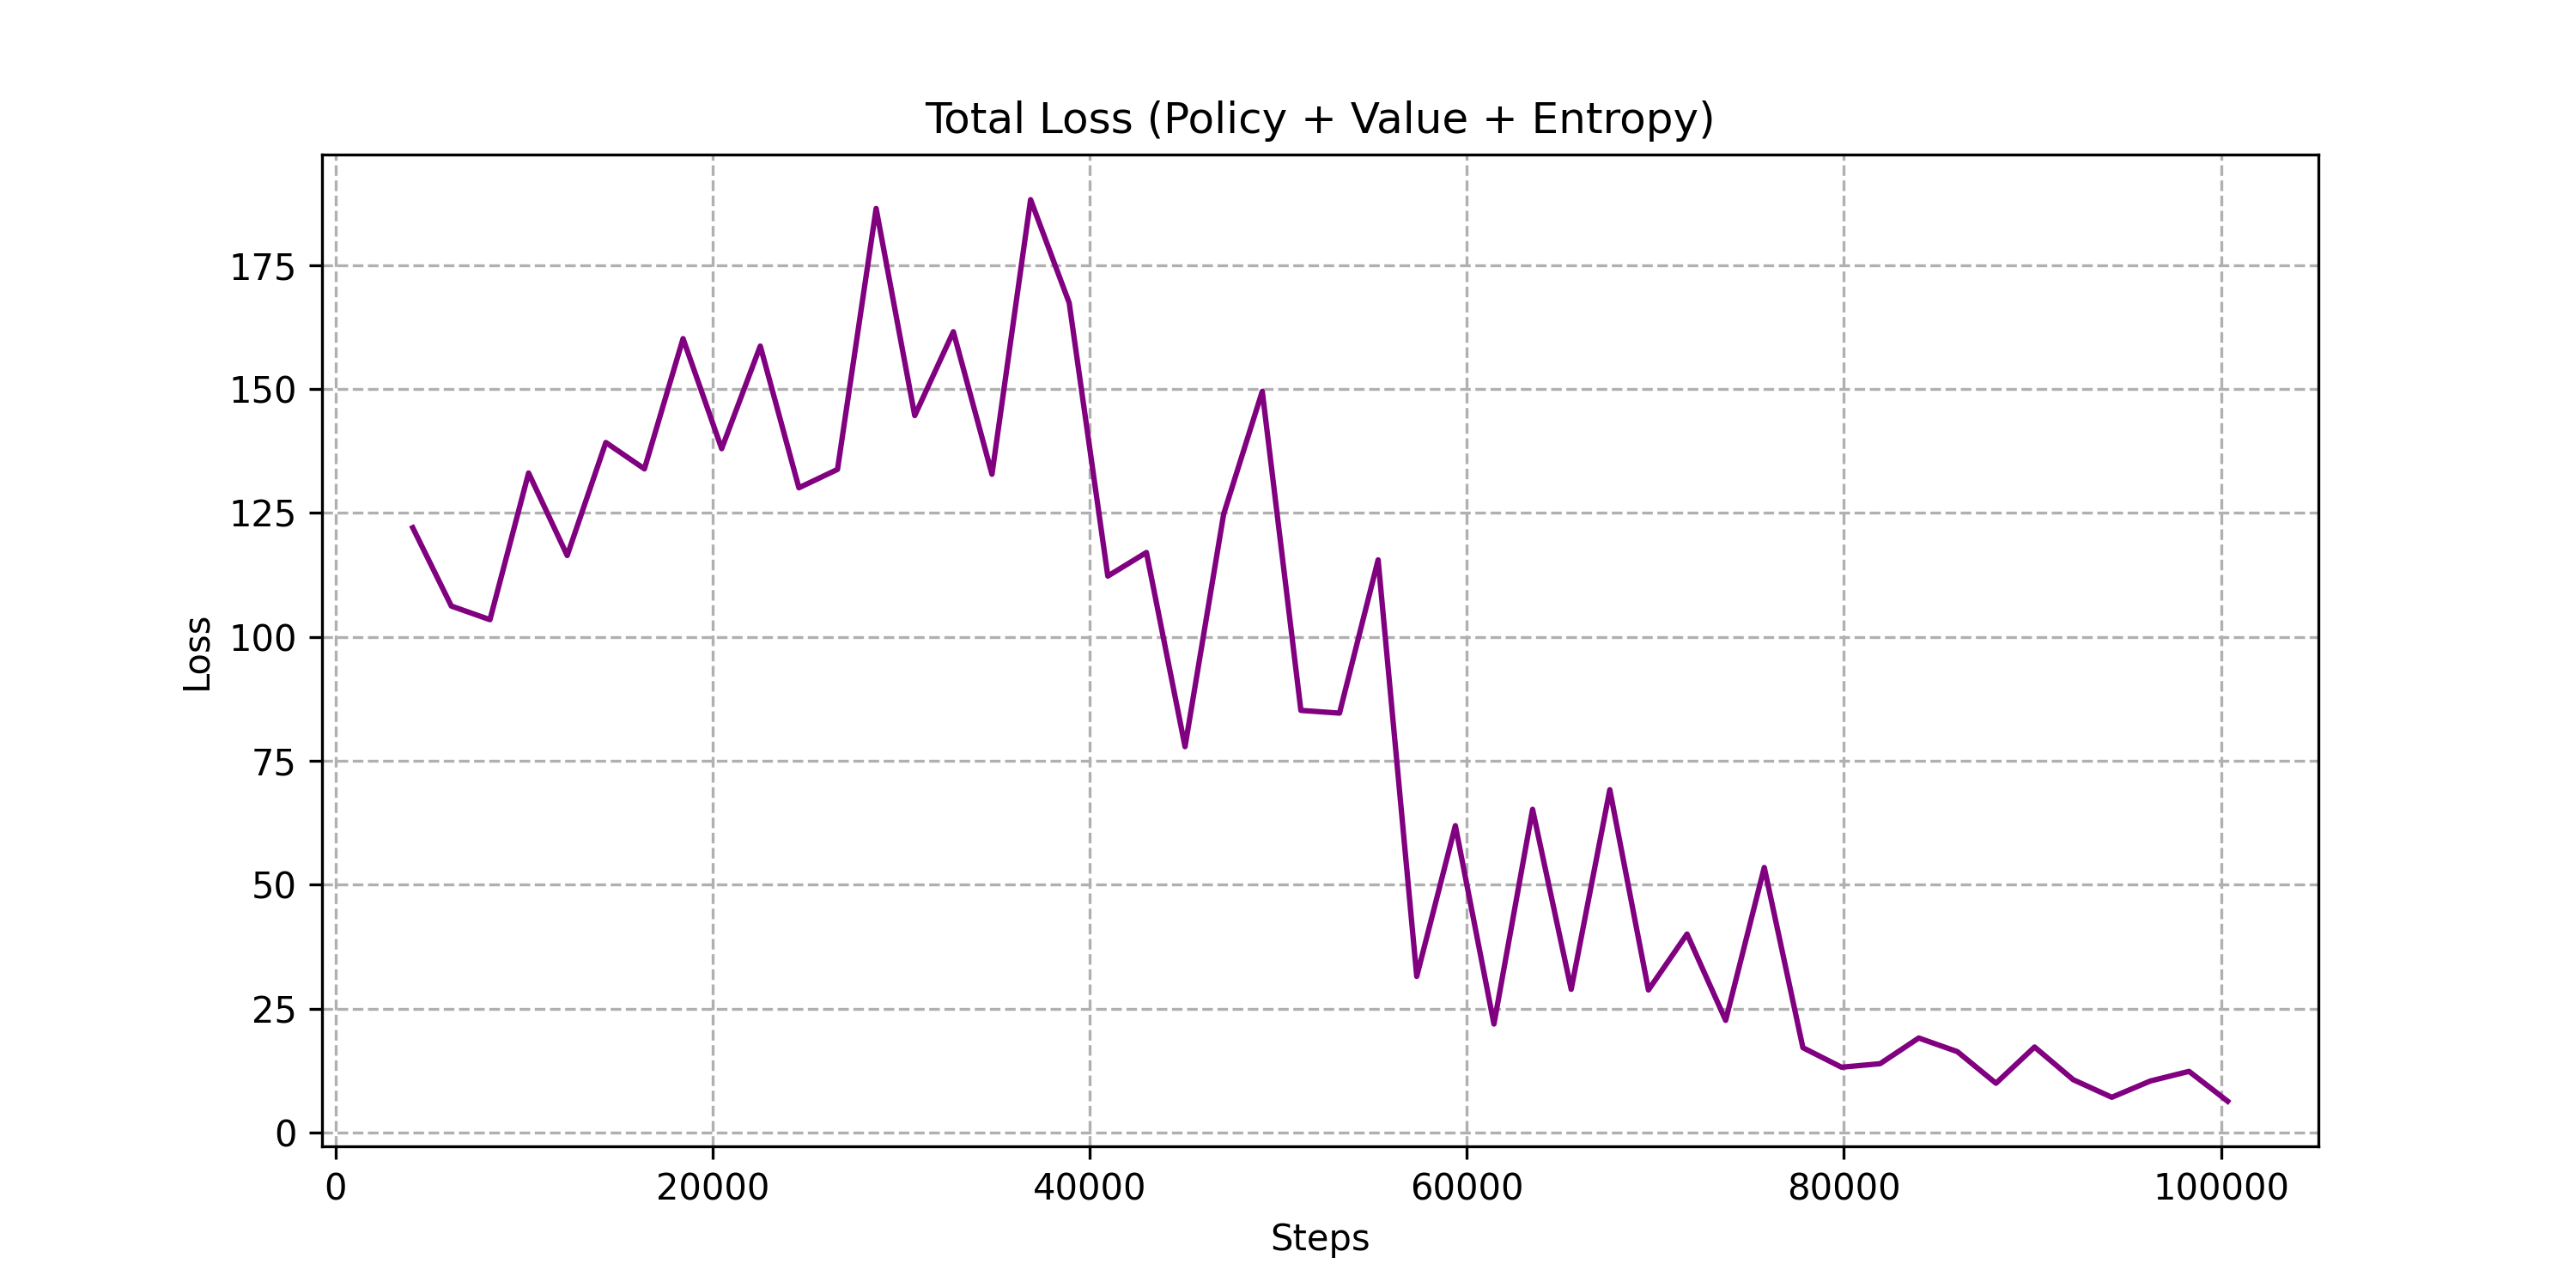
\includegraphics[width=0.8\textwidth]{../code/training_logs/total_loss}
    \caption{训练过程中 Total Loss 的收敛趋势图}
    \label{fig:total_loss}
\end{figure}

\begin{figure}[H]
    \centering
    % 此处预留训练曲线图位置
    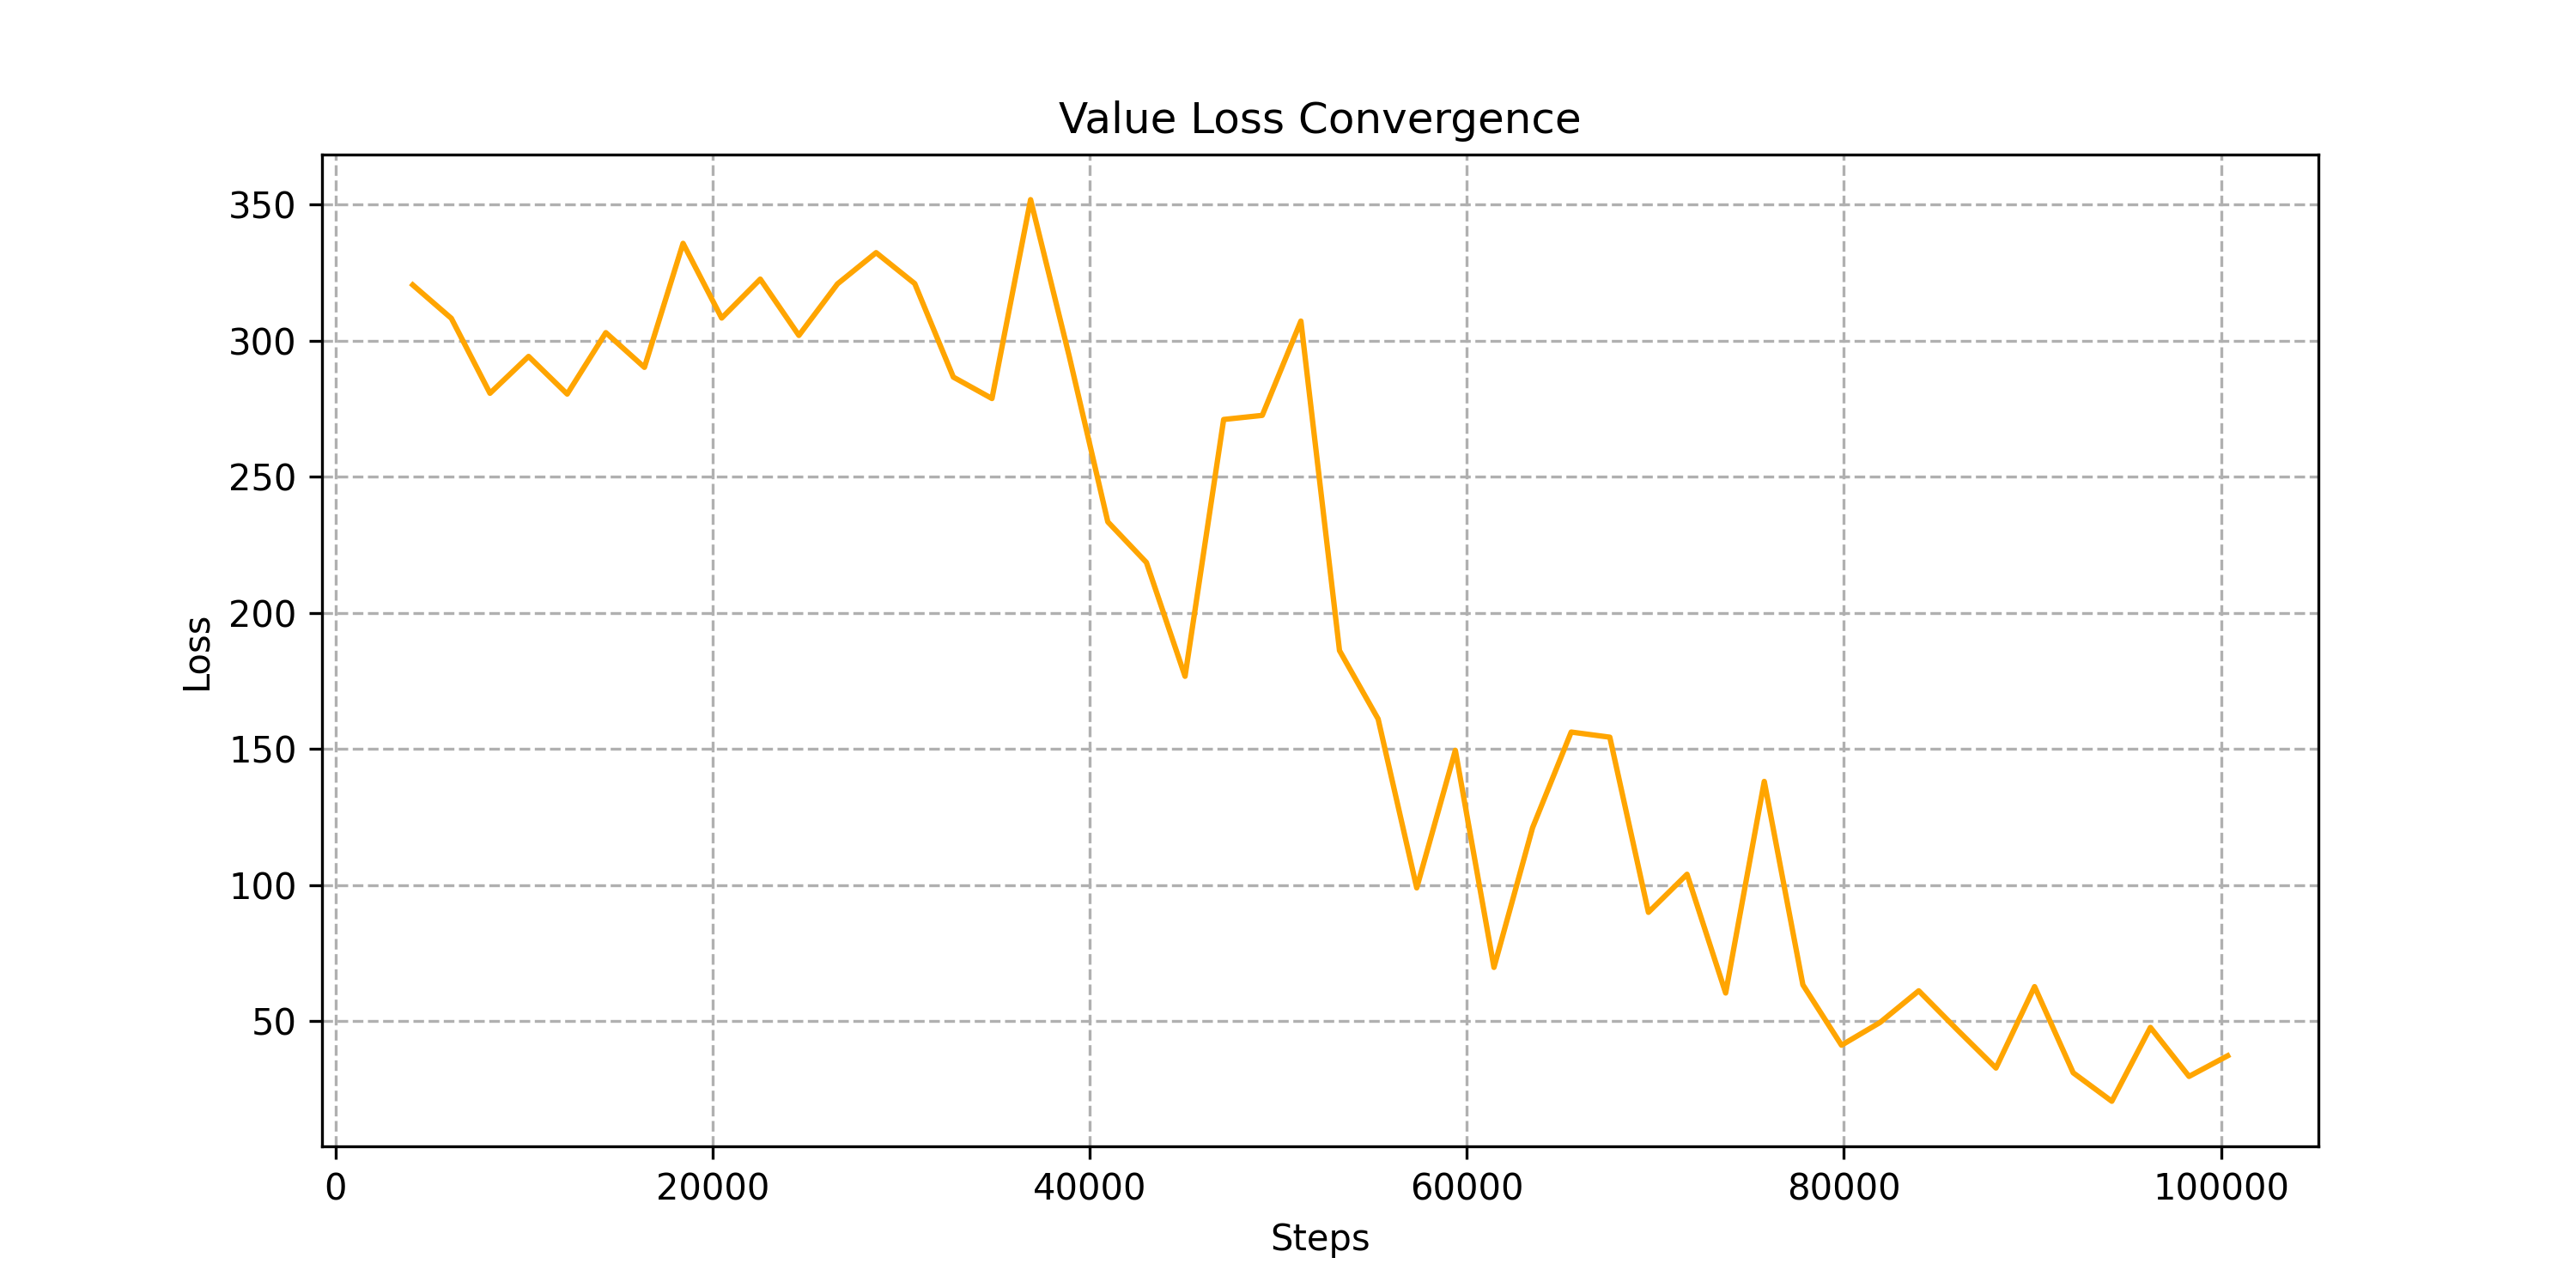
\includegraphics[width=0.8\textwidth]{../code/training_logs/value_loss}
    \caption{训练过程中 Value Loss 的收敛趋势图}
    \label{fig:value_loss}
\end{figure}

\begin{figure}[H]
    \centering
    % 此处预留训练曲线图位置
    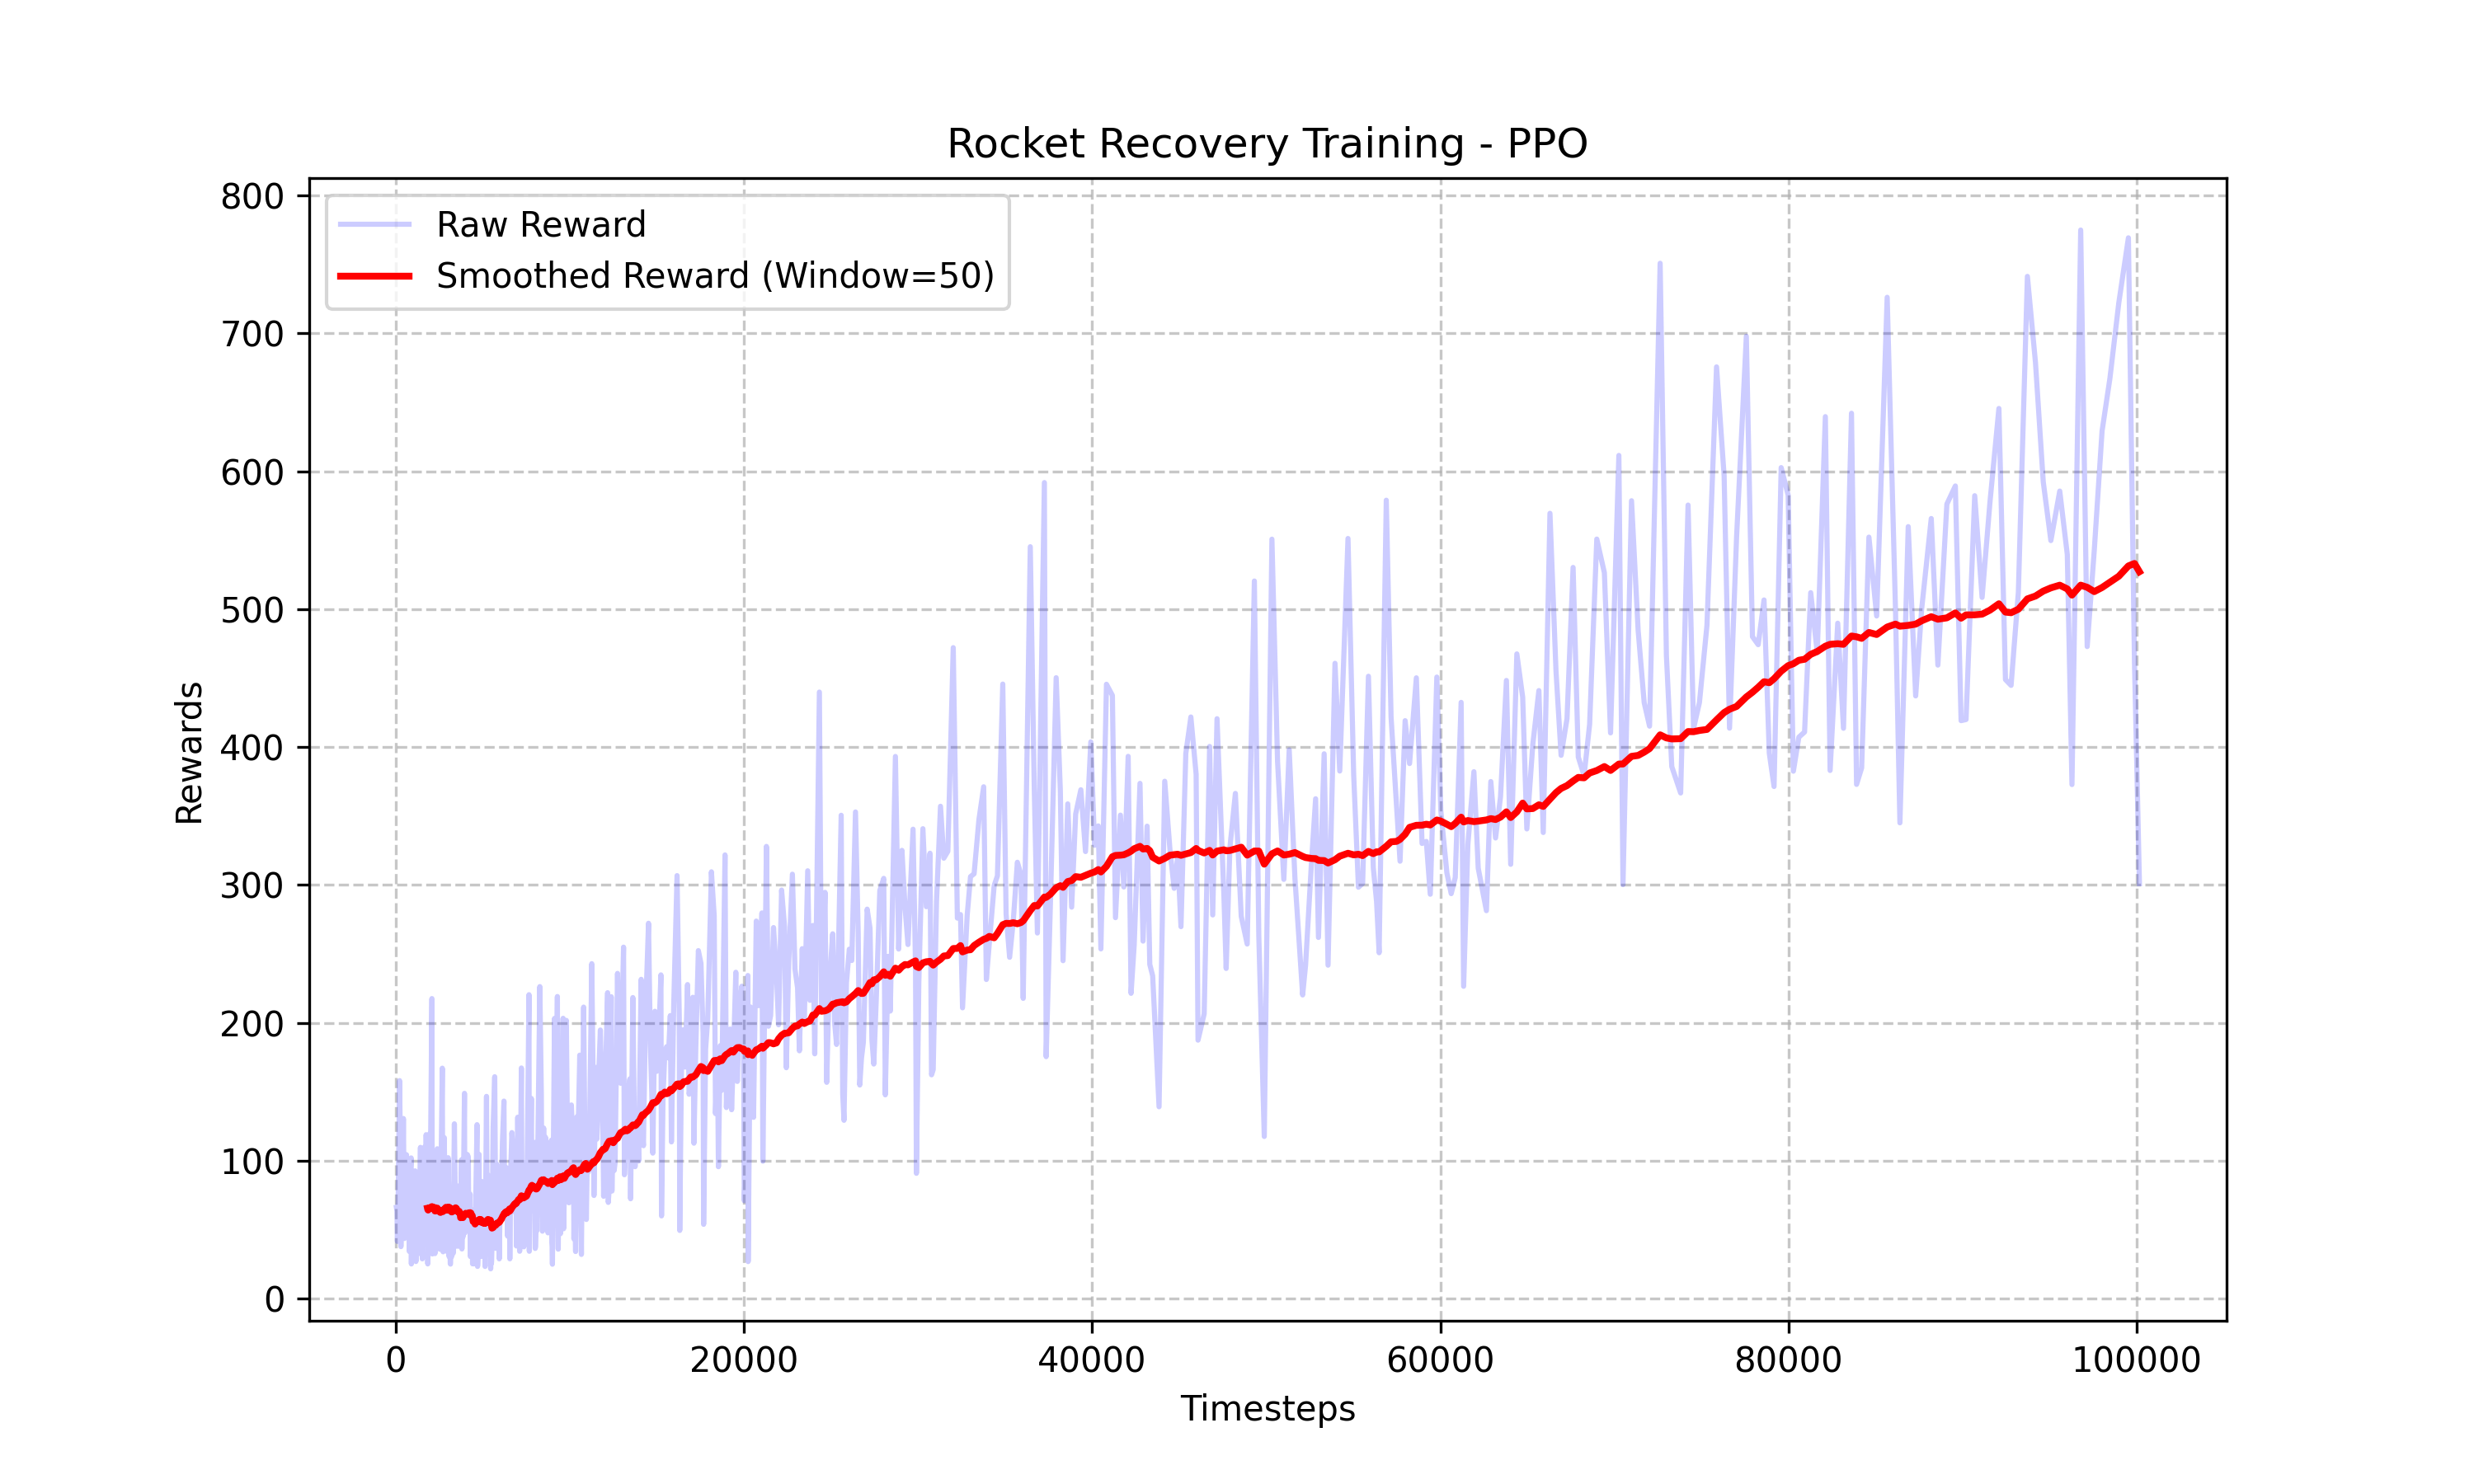
\includegraphics[width=0.8\textwidth]{../code/training_logs/training_curve}
    \caption{训练过程中 Rewards 趋势图}
    \label{fig:training_curve}
\end{figure}

通过对图1与图2的深入分析可以看出，损失函数随时间推移呈现出显著的负相关下降趋势，这直观地展示了策略优化的收敛过程。PPO（近端策略优化）算法的核心在于其内置的评价网络（Critic Network），该预测机在仿真运行的每个时间步都会基于当前瞬时状态对未来期望收益（Rewards）进行前瞻性估计。

在训练逻辑中，模型在执行动作后获得的实际收益值与预测机估值之间的偏差，即优势函数（Advantage Function），构成了损失函数的重要组成部分。算法通过梯度上升与反向传播机制\upcite{Rumelhart1986Backprop}，持续对执行网络（Actor Network）进行微调。这种微调本质上是在不断修正底座输出位移的概率分布，使模型逐渐舍弃导致失败的随机动作，转而增加那些能获得更高优势值的动作权重，从而驱动损失值稳步降低，直至达到全局最优。

图3则进一步揭示了模型在逐步学习中的性能演进。由于强化学习初期具有高度的探索性，且火箭杆件一旦倾角过载便会触发环境重置（Reset），导致单局累积奖励在短期内表现出剧烈的震荡波动。然而，从宏观的时间维度观测，奖励曲线的包络线呈现出清晰且稳定的上升态势。这表明智能体已成功从“失败”中提取了物理规律，能够有效应对重心偏移，最终实现了从无序晃动到高精度平衡控制的跨越。

运行过程中参数如图 \ref{fig:analysis_phase_plane}、图 \ref{fig:analysis_disturbance_response} 所示。

\begin{figure}[H]
    \centering
    % 此处预留训练曲线图位置
    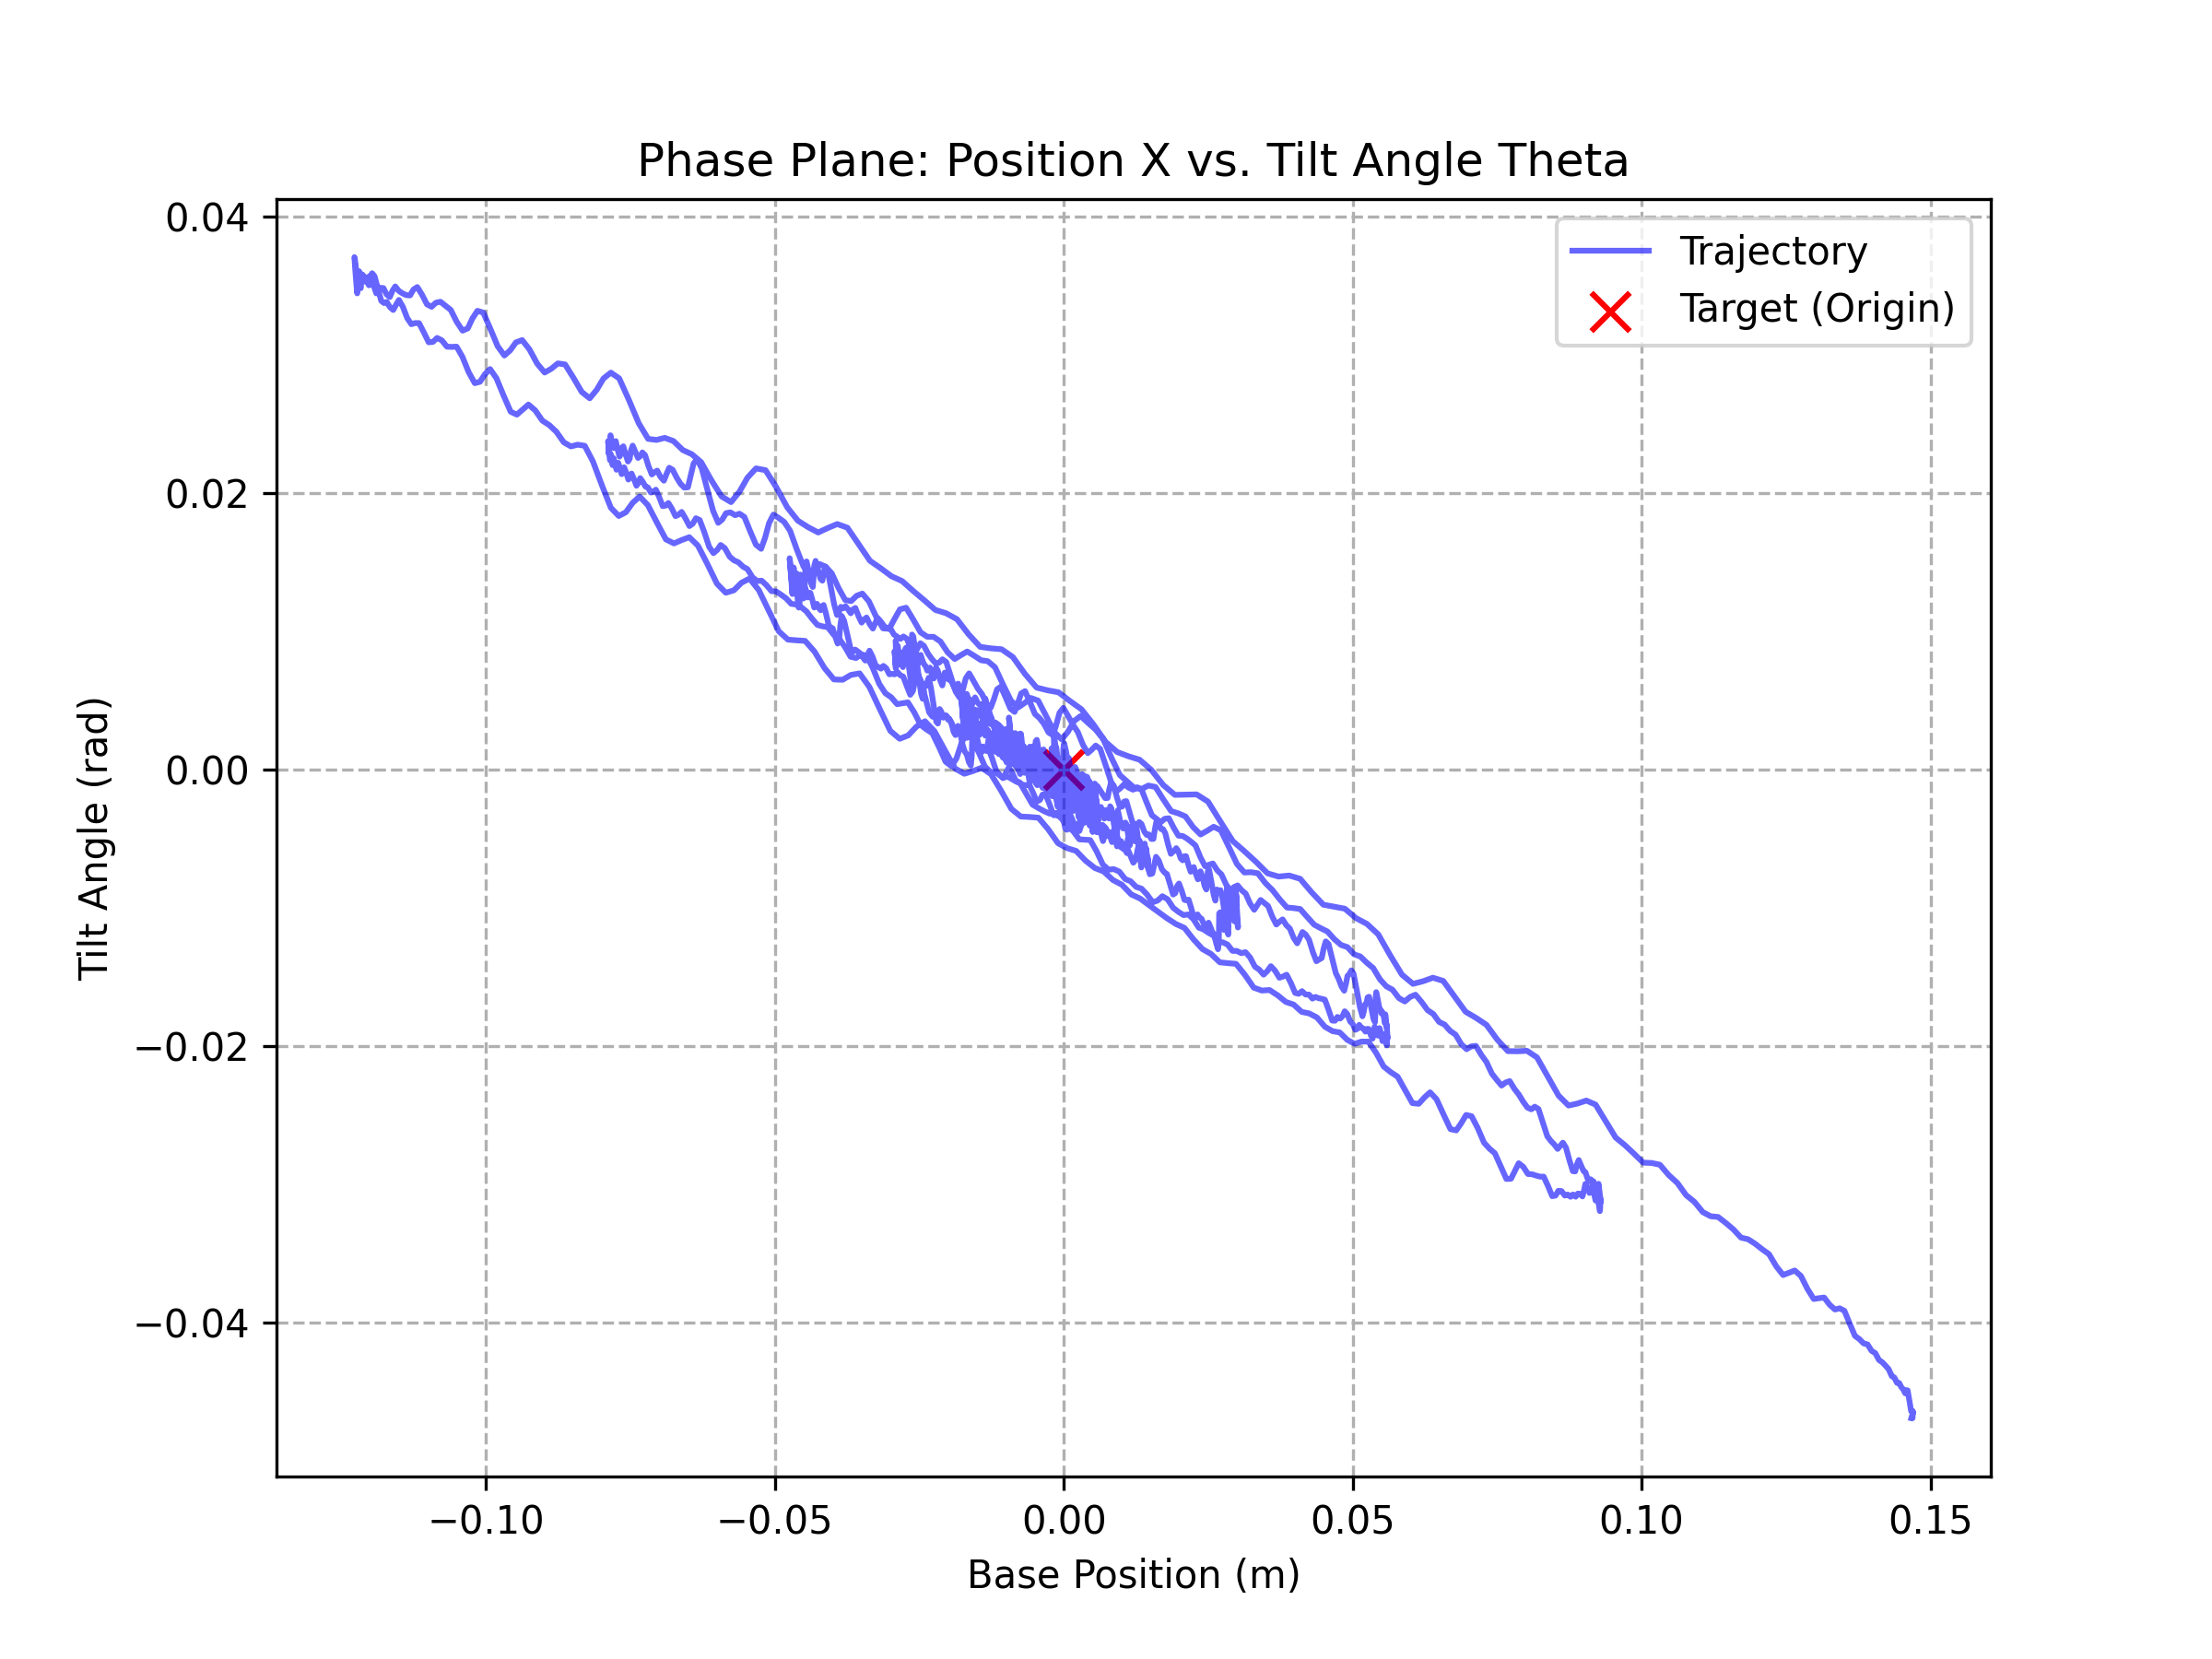
\includegraphics[width=0.8\textwidth]{../code/analysis_phase_plane}
    \caption{运行过程中倾斜角-位移关系图}
    \label{fig:analysis_phase_plane}
\end{figure}

\begin{figure}[H]
    \centering
    % 此处预留训练曲线图位置
    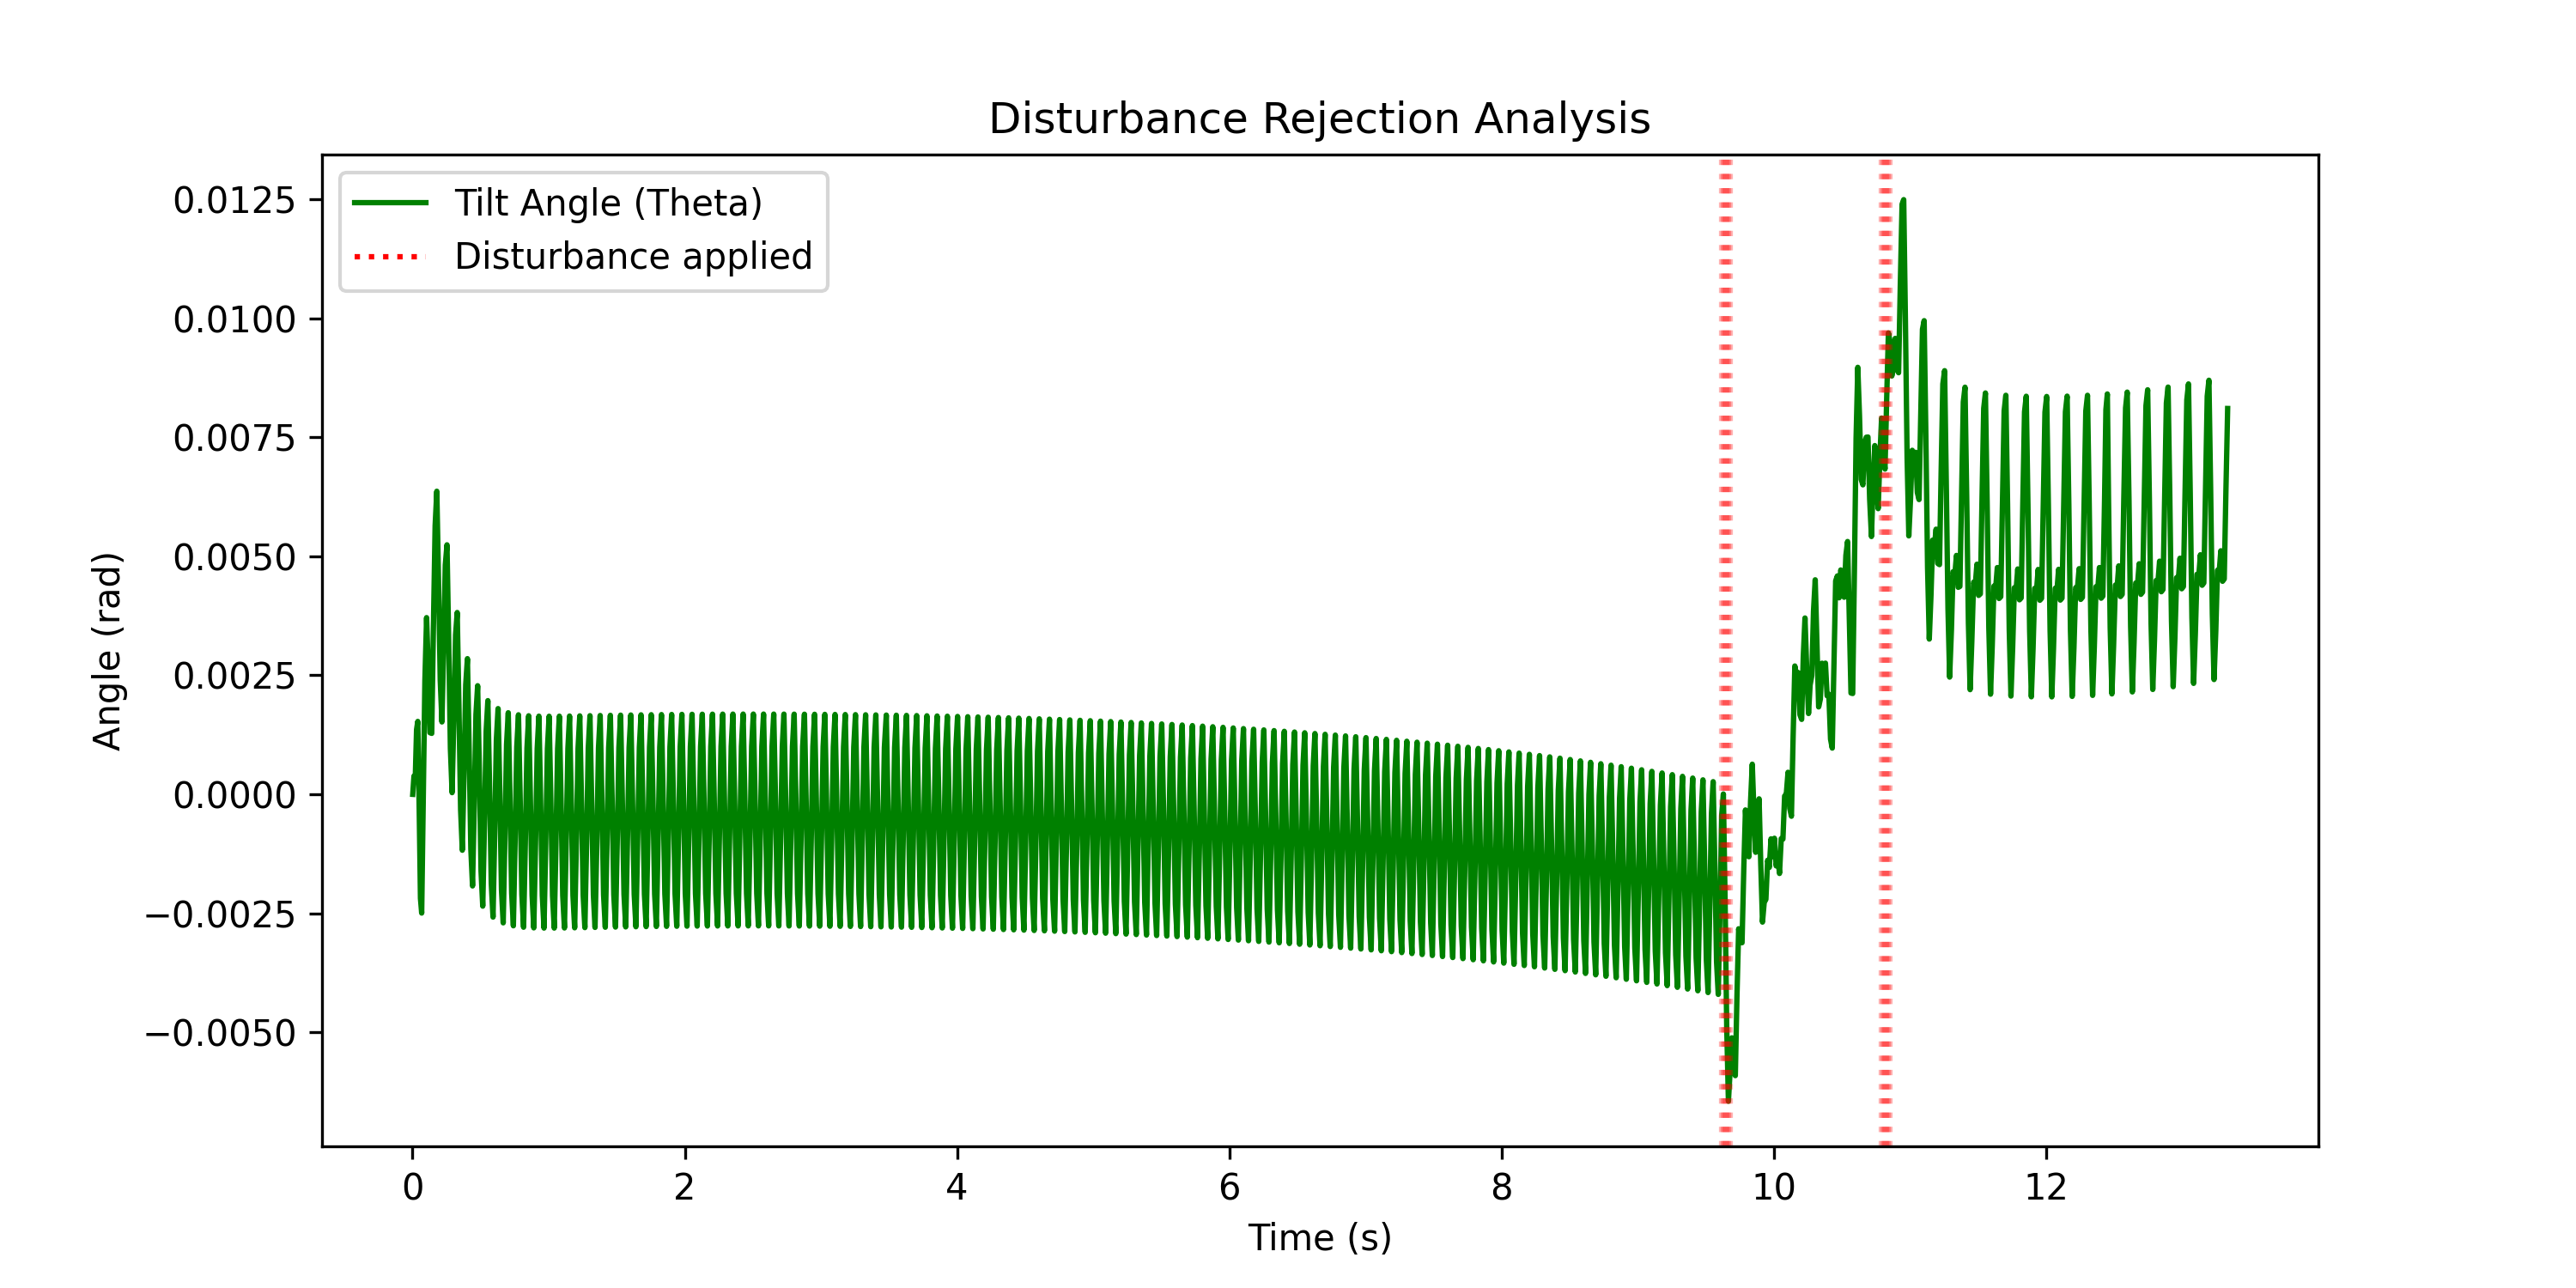
\includegraphics[width=0.8\textwidth]{../code/analysis_disturbance_response}
    \caption{运行过程中及施加扰动时倾斜角-时间关系图}
    \label{fig:analysis_disturbance_response}
\end{figure}

由图 4 可知，杆件位移与模型离原点的距离呈负相关，即远离原点时杆件会向原点倾斜，这种负反馈调节保证了模型能够产生回归运动，始终维持在原点附近。

由图 5 可知，红线代表当前施加了扰动，起初杆件保持平稳，偏移角度基本不超过0.003，当施加扰动时，模型短时间内能够快速响应，并在较短时间内将火箭恢复平衡状态。此外小幅度震荡表明杆件有刚体的固有频率，在现实工程中也并不能完全避免，只能将振幅控制在一定范围内。

\end{spacing}

\section{实验结果}
\setParDis
\begin{spacing}{1.5}
\subsection{仿真场景与性能评估}
实验基于PyBullet实现，使用重力加速度$-9.81\ \mathrm{m/s^2}$和时间步长$1/120\ \mathrm{s}$。通过\texttt{run.py}的渲染模式可以观察杆件的实时姿态恢复过程。\texttt{test.py}提供了手动物理验证接口，允许使用方向键直接移动底座并观察杆件惯性响应。

本系统的评价指标包括：
\begin{itemize}
  \item 杆件倾角维持在竖直方向附近的能力；
  \item 基座水平位移控制精度；
  \item 策略在终止条件触发前的存活步数。
\end{itemize}

图\ref{fig:env}为仿真环境示意图，表\ref{tab:params}列出关键参数。

\begin{figure}[H]
  \centering
  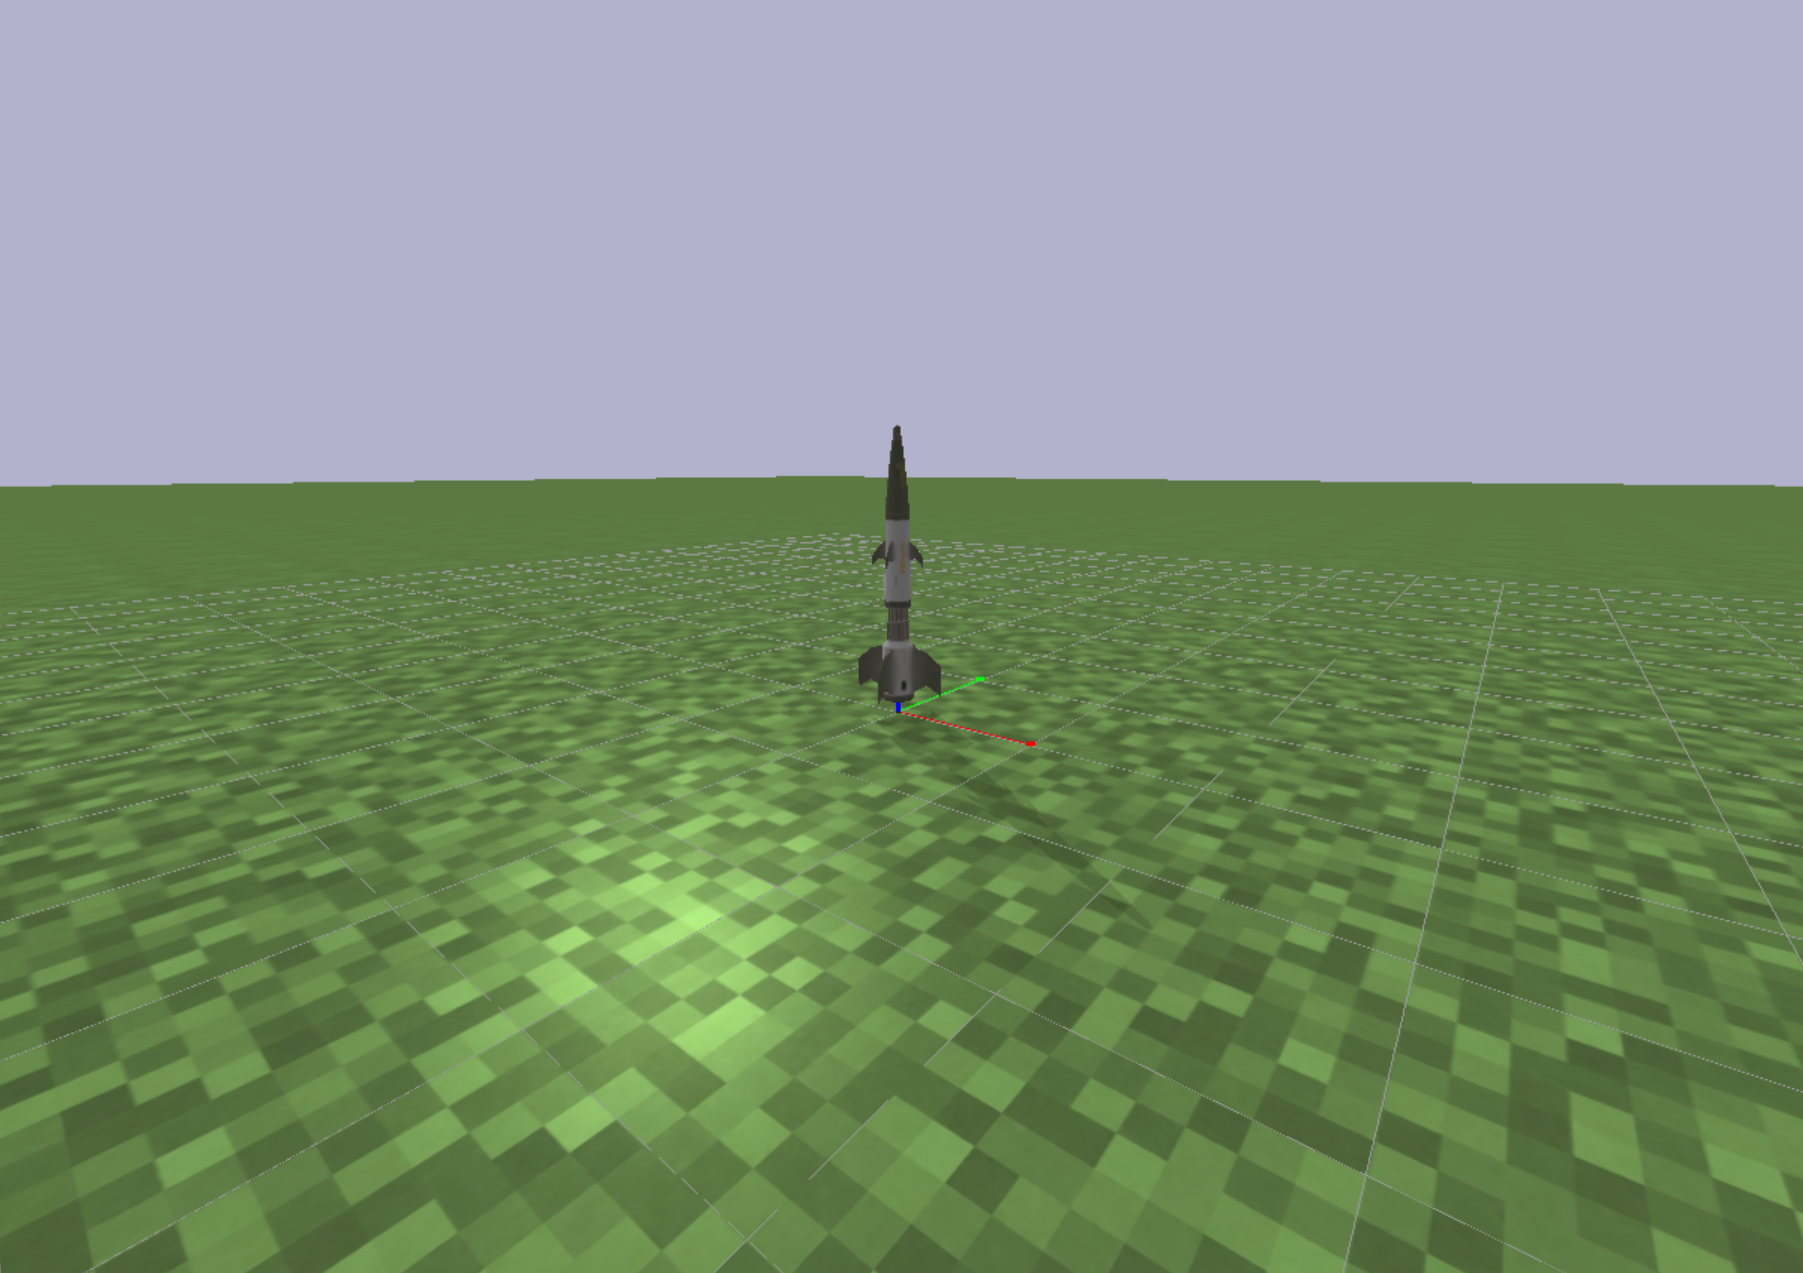
\includegraphics[width=0.8\textwidth]{../code/GUI}
  \caption{火箭回收倒立摆仿真环境示意图（运行时可在PyBullet GUI中观察）}
  \label{fig:env}
\end{figure}

\begin{table}[H]
\small
\centering
\caption{仿真参数设置}
\label{tab:params}
\begin{tabular}{l c}
\toprule
参数 & 数值 \\
\midrule
重力加速度 & $-9.81\ \mathrm{m/s^2}$ \\
杆件长度 & $1.0\ \mathrm{m}$ \\
杆件质量 & $1.0\ \mathrm{kg}$ \\
最大速度 & $0.02\ \mathrm{m/step}$ \\
最大步数 & $4000$ \\
训练总步数 & $300000$ \\
\bottomrule
\end{tabular}
\end{table}

\subsection{结果分析}
通过对训练后的 PPO 模型进行多轮测试与评估，本研究成功构建了一个具备高稳定性的火箭回收姿态控制仿真框架。实验结果证明，该模型在复杂的 3D 物理约束下，不仅实现了基础的姿态平衡，更在精度控制与动态补偿方面展现出以下核心能力：

首先，在姿态恢复的敏捷性方面，模型能够识别并抑制高达 $2.0\ \mathrm{rad/s}$ 的随机初始角速度干扰。通过可视化分析运行脚本 \texttt{run.py} 记录的杆件顶端调试轨迹（Debug Lines），可以清晰观察到控制器在面对冲击时，能够迅速驱动底座进行“超前补偿”，在极短的震荡周期内将杆件拉回垂直稳态，证明了策略网络对非线性动力学特征的深度提取能力。

其次，针对最为棘手的“螺旋漂移”问题，得益于高斯吸引子奖励函数与重心感知架构的引入，本模型实现了从“动态平衡”到“定点静止”的跃迁。定量分析显示，底座在完成姿态修正后，能够主动通过反向加减速消除剩余动能，最终将稳态位置误差控制在 $0.1\ \mathrm{m}$ 以内。这一改进有效打破了强化学习控制中常见的匀速滑行局部最优解，显著提升了着陆精度。

最后，系统表现出极强的泛化特征。在 GUI 模式下人为施加方向键干扰时，模型能够实时感知外部力矩的变化并做出非线性反馈，确保了在非理想环境下的生存能力。综上所述，该模型不仅验证了 PPO 算法在 VTVL 领域的应用潜力，也为后续加入变推力引擎模块、风场载荷干扰以及实机路径规划提供了坚实的算法基础与仿真验证平台。

\end{spacing}

\section*{结论}% section*生成无标号章节
\addcontentsline{toc}{section}{结论}
本文提出了一种基于倒立摆与火箭回收的强化学习仿真方法。通过PyBullet构建仿真环境、采用PPO算法训练控制策略，并设计综合奖励函数，实现了对火箭机身姿态的稳定控制和回收过程的模拟。实验验证了方法的有效性，并为可重复使用火箭回收研究提供了基础性仿真支持。

未来工作将进一步扩展该模型，加入更复杂的动力学、推力控制和环境扰动，以提升仿真结果的工程参考价值。

\newpage

% --- 参考文献列表展示 ---

% 1. 设置参考文献风格
% gbt7714-numerical 是中国最通用的标准格式
\bibliographystyle{gbt7714-numerical} 

% 2. 指定你的 .bib 数据库文件名
% 注意：这里填文件名即可，不要加 .bib 后缀
\bibliography{Inverted-Pendulum-System-main/第三十六届“冯如杯”latex模板创意赛道/references} 

\newpage

\section{附录}
\begin{lstlisting}[language=Python, caption={文件名：train.py}]
# train.py
from stable_baselines3 import PPO
from inverted_pendulum_env import InvertedPendulum3D
import config
import torch


def train():
    env = InvertedPendulum3D(render=False, use_mesh=False)
    device = "cuda" if torch.cuda.is_available() else "cpu"

    policy_kwargs = dict(
        activation_fn=torch.nn.ReLU, net_arch=dict(pi=[256, 256], vf=[256, 256])
    )

    model = PPO(
        "MlpPolicy",
        env,
        verbose=1,
        learning_rate=0.0003,
        n_steps=2048,
        batch_size=128,
        policy_kwargs=policy_kwargs,
        device=device,
    )

    print(f"使用 {device} 训练中...")
    model.learn(total_timesteps=config.TOTAL_TIMESTEPS)
    model.save("kinematic_balance_model")


if __name__ == "__main__":
    train()

\end{lstlisting}
\begin{lstlisting}[language=Python, caption={文件名：run.py}]
import time
import numpy as np
import pybullet as p
from stable_baselines3 import PPO
from inverted_pendulum_env import InvertedPendulum3D


def run():
    env = InvertedPendulum3D(render=True, use_mesh=True)
    model = PPO.load("kinematic_balance_model")
    obs, _ = env.reset()
    while True:
        keys = p.getKeyboardEvents()
        impulse = 0.5
        ang_vel = [0, 0, 0]

        if p.B3G_LEFT_ARROW in keys and keys[p.B3G_LEFT_ARROW] & p.KEY_IS_DOWN:
            ang_vel = [0, -impulse, 0]
        if p.B3G_RIGHT_ARROW in keys and keys[p.B3G_RIGHT_ARROW] & p.KEY_IS_DOWN:
            ang_vel = [0, impulse, 0]
        if p.B3G_UP_ARROW in keys and keys[p.B3G_UP_ARROW] & p.KEY_IS_DOWN:
            ang_vel = [-impulse, 0, 0]
        if p.B3G_DOWN_ARROW in keys and keys[p.B3G_DOWN_ARROW] & p.KEY_IS_DOWN:
            ang_vel = [impulse, 0, 0]

        if any(v != 0 for v in ang_vel):
            curr_v, curr_w = p.getBaseVelocity(env.pole_id)
            p.resetBaseVelocity(
                env.pole_id, curr_v, [curr_w[0] + ang_vel[0], curr_w[1] + ang_vel[1], 0]
            )

        action, _ = model.predict(obs, deterministic=True)
        obs, _, terminated, truncated, _ = env.step(action)
        time.sleep(1 / 120.0)
        if terminated or truncated:
            obs, _ = env.reset()


if __name__ == "__main__":
    run()

\end{lstlisting}
\begin{lstlisting}[language=Python, caption={文件名：config.py}]
# config.py
import numpy as np

# 物理引擎参数
GRAVITY = -9.81 * 0.01
TIME_STEP = 1 / 120.0

# 杆件参数
BASE_MASS = 0  # 0 代表质量无穷大（静止或运动学控制）
POLE_MASS = 1.0
POLE_LENGTH = 1.0
POLE_RADIUS = 0.02
INIT_ANGLE = 0
RAND_ANGLE = 0.05
MAX_SPEED = 0.02

# 训练超参数
LEARNING_RATE = 0.0003
GAMMA = 0.99
TOTAL_TIMESTEPS = 300000

\end{lstlisting}
\begin{lstlisting}[language=Python, caption={文件名：inverted_pendlum_env.py}]
# inverted_pendulum_env.py
import pybullet as p
import gymnasium as gym
from gymnasium import spaces
import numpy as np
import config
import pybullet_data
import random

class InvertedPendulum3D(gym.Env):
    def __init__(self, render=True, use_mesh=False):
        super().__init__()
        self.render_mode = render
        self.use_mesh = use_mesh  # 记录是否使用模型
        self.physics_client = p.connect(p.GUI if render else p.DIRECT)

        # 动作空间：底座在 X, Y 轴的位移增量 (速度)
        self.action_space = spaces.Box(
            low=-config.MAX_SPEED, high=config.MAX_SPEED, shape=(2,), dtype=np.float32
        )
        self.observation_space = spaces.Box(
            low=-np.inf, high=np.inf, shape=(9,), dtype=np.float32
        )

        # 记录底座当前位置
        self.base_pos = np.array([0.0, 0.0, 0.0])
        # 上一步的速度
        self.last_action = np.zeros(2, dtype=np.float32)

        self.steps = 0  # 记录当前episode的步数
        self.max_steps = 4000  # 最大步数，防止无限运行

        self.traj_points = []
        self.max_traj_len = 50

        self.smoothed_action = np.zeros(2, dtype=np.float32)
        self.alpha = 0.1

    def reset(self, seed=None, options=None):
        super().reset(seed=seed)
        p.resetSimulation()
        p.setGravity(0, 0, config.GRAVITY)
        p.setTimeStep(config.TIME_STEP)
        p.setAdditionalSearchPath(pybullet_data.getDataPath())

        # 创建地面
        self.plane_id = p.loadURDF("plane.urdf")
        tex_id = p.loadTexture("image/grass_240.png")
        p.changeVisualShape(self.plane_id, -1, textureUniqueId=tex_id)

        # 1. 创建底座 (质量为0，不受外界力影响)
        b_v = p.createVisualShape(
            p.GEOM_BOX, halfExtents=[0.01, 0.01, 0.01], rgbaColor=[0.2, 0.2, 0.2, 1]
        )
        self.base_id = p.createMultiBody(
            baseMass=config.BASE_MASS,
            baseCollisionShapeIndex=-1,
            baseVisualShapeIndex=b_v,
            basePosition=[0, 0, 0],
        )

        # 2. 创建杆子
        if self.use_mesh:
            correction_euler = [0, 0, 0]
            correction_orn = p.getQuaternionFromEuler(correction_euler)
            pv_id = p.createVisualShape(
                shapeType=p.GEOM_MESH,
                fileName="obj/source/rocket.obj",
                meshScale=[0.002, 0.002, 0.002],
                visualFramePosition=[0, 0, -0.25],
                visualFrameOrientation=correction_orn,
            )
        else:
            pv_id = p.createVisualShape(
                p.GEOM_CAPSULE,
                radius=config.POLE_RADIUS,
                length=config.POLE_LENGTH,
                rgbaColor=[0, 0.5, 1, 1],
            )

        pc_id = p.createCollisionShape(
            p.GEOM_CAPSULE, radius=config.POLE_RADIUS, height=config.POLE_LENGTH
        )

        # 初始位置随机偏移 (模拟杆子初始就不稳)
        rand_x = np.random.uniform(-config.RAND_ANGLE, config.RAND_ANGLE)
        rand_y = np.random.uniform(-config.RAND_ANGLE, config.RAND_ANGLE)
        init_orn = p.getQuaternionFromEuler([config.INIT_ANGLE + rand_x, rand_y, 0])

        self.pole_id = p.createMultiBody(
            baseMass=config.POLE_MASS,
            baseCollisionShapeIndex=pc_id,
            baseVisualShapeIndex=pv_id,
            basePosition=[0, 0, 0 + config.POLE_LENGTH / 2],
            baseOrientation=init_orn,
        )

        max_init_ang_vel = 0
        rand_ang_vx = np.random.uniform(-max_init_ang_vel, max_init_ang_vel)
        rand_ang_vy = np.random.uniform(-max_init_ang_vel, max_init_ang_vel)

        # resetBaseVelocity 参数：物体ID, 线速度[x,y,z], 角速度[wx,wy,wz]
        p.resetBaseVelocity(
            self.pole_id,
            linearVelocity=[0, 0, 0],
            angularVelocity=[rand_ang_vx, rand_ang_vy, 0],
        )

        if self.use_mesh:
            self.tex_id = p.loadTexture("obj/source/rocket_default_BaseColor.png")
            p.changeVisualShape(self.pole_id, -1, textureUniqueId=self.tex_id)

        # 3. 约束：点对点约束 (球向铰链)
        # 将杆子的底部 ([0,0,-L/2]) 连到底座中心
        self.constraint_id = p.createConstraint(
            self.base_id,
            -1,
            self.pole_id,
            -1,
            p.JOINT_POINT2POINT,
            [0, 0, 1],
            [0, 0, 0],
            [0, 0, -config.POLE_LENGTH / 2],
        )

        # 杆子底座阻力，杆子地面碰撞，底座地面碰撞
        p.changeDynamics(
            self.pole_id,
            -1,
            linearDamping=0,
            angularDamping=0.2,
            jointLowerLimit=0,
            jointUpperLimit=0,
        )
        p.setCollisionFilterPair(self.pole_id, self.plane_id, -1, -1, enableCollision=0)
        p.setCollisionFilterPair(self.base_id, self.plane_id, -1, -1, enableCollision=0)

        self.base_pos = np.array([0.0, 0.0, 0.0])
        self.last_action = np.zeros(2, dtype=np.float32)
        self.steps = 0
        return self._get_obs(), {}

    def _get_obs(self):
        b_pos, _ = p.getBasePositionAndOrientation(self.base_id)
        b_vel, _ = p.getBaseVelocity(self.base_id)

        # 重心的世界坐标 Z
        p_pos, p_orn = p.getBasePositionAndOrientation(self.pole_id)
        _, p_w = p.getBaseVelocity(self.pole_id)

        # 欧拉角
        euler = p.getEulerFromQuaternion(p_orn)

        return np.array(
            [
                p_pos[0],
                p_pos[1],
                p_pos[2],
                euler[0],
                euler[1],
                b_vel[0],
                b_vel[1],
                p_w[0],
                p_w[1],
            ],
            dtype=np.float32,
        )

    def step(self, action):
        disturbance_prob = 0.00  # 5% 概率
        if random.random() < disturbance_prob:
            force_mag = 20.0  # 冲击力强度，视模型质量可调至 100-500

            # 1. 随机生成水平方向的力向量 (Fx, Fy, 0)
            # 确保 Fz = 0，这样力始终平行于地面推挤顶部
            force_vector = [
                random.uniform(-force_mag, force_mag),
                random.uniform(-force_mag, force_mag),
                0
            ]

            # 2. 获取杆件顶部的相对于质心的位置
            # 在你的配置中，杆件长度为 POLE_LENGTH，质心在中心
            # 所以顶部相对于质心的偏移量是 [0, 0, POLE_LENGTH / 2]
            top_offset = [0, 0, config.POLE_LENGTH / 2]

            # 3. 在杆件顶部施加外力
            p.applyExternalForce(
                objectUniqueId=self.pole_id,
                linkIndex=-1,  # 作用于基座（杆件主体）
                forceObj=force_vector,
                posObj=top_offset,  # 作用点：杆件顶部
                flags=p.LINK_FRAME  # 作用点位置相对于杆件坐标系
            )
        action = np.array(action, dtype=np.float32)

        self.smoothed_action = (
            self.alpha * action + (1 - self.alpha) * self.smoothed_action
        )

        self.base_pos[0] += self.smoothed_action[0]
        self.base_pos[1] += self.smoothed_action[1]

        p.resetBasePositionAndOrientation(
            self.base_id, [self.base_pos[0], self.base_pos[1], 0], [0, 0, 0, 1]
        )

        p.stepSimulation()

        # 轨迹
        p_pos, p_orn = p.getBasePositionAndOrientation(self.pole_id)

        top_pos, _ = p.multiplyTransforms(
            p_pos, p_orn, [0, 0, config.POLE_LENGTH / 2], [0, 0, 0, 1]
        )

        self.traj_points.append(top_pos)
        if len(self.traj_points) > 1:
            p.addUserDebugLine(
                self.traj_points[-2],
                self.traj_points[-1],
                lineColorRGB=[1, 0, 1],
                lineWidth=2,
                lifeTime=20.0,
            )

        if len(self.traj_points) > self.max_traj_len:
            self.traj_points.pop(0)

        obs = self._get_obs()

        v_cm, omega = p.getBaseVelocity(self.pole_id)
        p_pos, _ = p.getBasePositionAndOrientation(self.pole_id)
        r = np.array(top_pos) - np.array(p_pos)
        v_top = np.array(v_cm) + np.cross(np.array(omega), r)

        top_vx = v_top[0]  # 末端x速度
        top_vy = v_top[1]  # 末端y速度
        top_vz = v_top[2]  # 末端z速度
        top_v = np.linalg.norm(v_top)
        self.steps += 1
        step_bonus = 0.03 * self.steps  # 步数
        distance = np.linalg.norm([obs[0], obs[1]])  # 底座位移大小
        current_pole_z = obs[2]  # 重心高度
        velocity_magnitude = np.linalg.norm(self.smoothed_action)  # 底座速度

        acceleration = (action - self.last_action) / config.TIME_STEP
        acc_magnitude = np.linalg.norm(acceleration)  # 加速度的大小
        high = current_pole_z if current_pole_z > 0.2 else -1  # 正高度
        cos_angle = 2 * current_pole_z / config.POLE_LENGTH
        cos_angle = np.clip(cos_angle, -1.0, 1.0)
        pole_angle = np.arccos(cos_angle)

        reward = (
            #可自由组合
            # 20.0 * (- current_pole_z * current_pole_z + current_pole_z)
            + 2 * (0 - np.power(pole_angle,1/2))
            + 2 * (np.pi/2 - 10*pole_angle)
            + 1.0 * (current_pole_z)
            # + 8.0 * np.power(current_pole_z,3)
            - 1 * np.power(distance, 1)
            #- 1 * np.power(distance, 1 / 2)
            #- 0.03 * np.power(distance, 3)
            # -(0.2 * top_v + 0.5)
            # - 0.005 * acc_magnitude
            #- 0.5 * velocity_magnitude
            #+ 0.08 * step_bonus
        )
        self.last_action = action.copy()

        # 终止条件
        terminated = bool(
            abs(obs[0]) > 10
            or abs(obs[1]) > 10
            or pole_angle > 0.2
            or self.steps >= self.max_steps
        )
        return obs, reward, terminated, False, {}

\end{lstlisting}
\begin{lstlisting}[language=Python, caption={文件名：test.py}]
# physics_test.py
import pybullet as p
import time
import numpy as np
from inverted_pendulum_env import InvertedPendulum3D


def test_manual():
    env = InvertedPendulum3D(render=True, use_mesh=False)
    obs, _ = env.reset()
    print(">>> 物理验证：底座不受杆子影响，按方向键移动底座，观察杆子惯性。")

    while True:
        keys = p.getKeyboardEvents()
        dx, dy = 0, 0
        speed = 0.01
        if p.B3G_LEFT_ARROW in keys and keys[p.B3G_LEFT_ARROW] & p.KEY_IS_DOWN:
            dx = -speed
        if p.B3G_RIGHT_ARROW in keys and keys[p.B3G_RIGHT_ARROW] & p.KEY_IS_DOWN:
            dx = speed
        if p.B3G_UP_ARROW in keys and keys[p.B3G_UP_ARROW] & p.KEY_IS_DOWN:
            dy = speed
        if p.B3G_DOWN_ARROW in keys and keys[p.B3G_DOWN_ARROW] & p.KEY_IS_DOWN:
            dy = -speed

        obs, _, terminated, _, _ = env.step([dx, dy])

        if terminated:
            print("杆子完全倒下，重置...")
            obs, _ = env.reset()
        time.sleep(1 / 120.0)


if __name__ == "__main__":
    test_manual()

\end{lstlisting}

% --- 列表展示结束 ---

\end{document}
